\documentclass[envcountsect,dvips]{beamer}

\setbeamertemplate{background canvas}[vertical shading][bottom=yellow!20,top=blue!10]
%\usetheme{Darmstadt}
\usetheme{Warsaw}
%\usefonttheme[onlysmall]{structurebold}

\usepackage{natbib}
\usepackage{bibentry}
\bibliographystyle{plain}
\usepackage{chngcntr}

\usepackage[utf8]{inputenc}
\usepackage{default}
\usepackage{amsmath}
\usepackage{amsfonts}
\usepackage{amssymb}

\usepackage{graphicx}
\usepackage{caption}
\usepackage{subcaption}

\usepackage{color,xcolor,ucs}% para textcolor



\newenvironment<>{varblock}[2][.9\textwidth]{%
  \setlength{\textwidth}{#1}
  \begin{actionenv}#3%
    \def\insertblocktitle{#2}%
    \par%
    \usebeamertemplate{block begin}}
  {\par%
    \usebeamertemplate{block end}%
  \end{actionenv}}

%%%%%%%%%%%%%%%%%%%%%%%%%%%%%%%%%%%%%%%%%%%%%%%%%%%%%%%%%%%%%%%%%%%%%%%%%%
\begin{document}

\title[Aritmética com inteiros:   ] % (optional, only for long titles)
{Aritmética com inteiros e}
\subtitle{Representação e ponto flutuante}
\author[Fernando] % (optional, for multiple authors)
{Fernando Pujaico Rivera\inst{1}}
\institute[Universidade Federal de Lavras] % (optional)
{
  \inst{1}%
  Universidade Federal de Lavras
}
\date[2016] % (optional)
{Aula-1 2016}
\subject{Computer Science}
\frame{\titlepage}

%%%%%%%%%%%%%%%%%%%%%%%%%%%%%%%%%%%%%%%%%%%%%%%%%%%%%%%%%%%%%%%%%%%%%%%%%%%%%%%%
%%%%%%%%%%%%%%%%%%%%%%%%%%%%%%%%%%%%%%%%%%%%%%%%%%%%%%%%%%%%%%%%%%%%%%%%%%%%%%%%
%%%%%%%%%%%%%%%%%%%%%%%%%%%%%%%%%%%%%%%%%%%%%%%%%%%%%%%%%%%%%%%%%%%%%%%%%%%%%%%%
\section{Aritmética com inteiros positivos}

%%%%%%%%%%%%%%%%%%%%%%%%%%%%%%%%%%%%%%%%%%%%%%%%%%%%%%%%%%%%%%%%%%%%%%%%%%%%%%%%%
\begin{frame}{Número inteiro positivo (decimal) $\rightarrow$ binário}
Divisões sucessivas por 2
\begin{center}
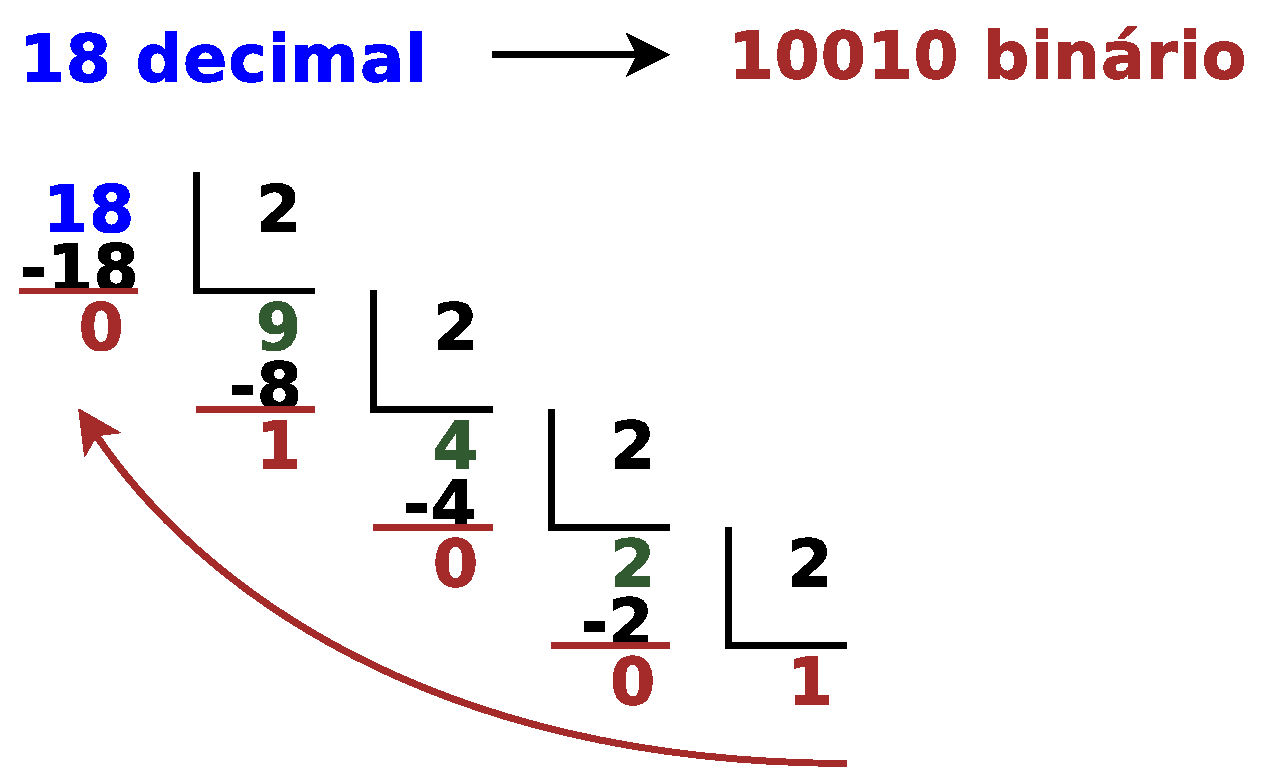
\includegraphics[width=0.6\textwidth]{images/decimal2binario.eps}
\end{center}
\end{frame}

%%%%%%%%%%%%%%%%%%%%%%%%%%%%%%%%%%%%%%%%%%%%%%%%%%%%%%%%%%%%%%%%%%%%%%%%%%%%%%%%%
\begin{frame}{Numero binário $\rightarrow$ inteiro positivo (decimal)}
\begin{minipage}[c]{0.6\textwidth}
\begin{center}
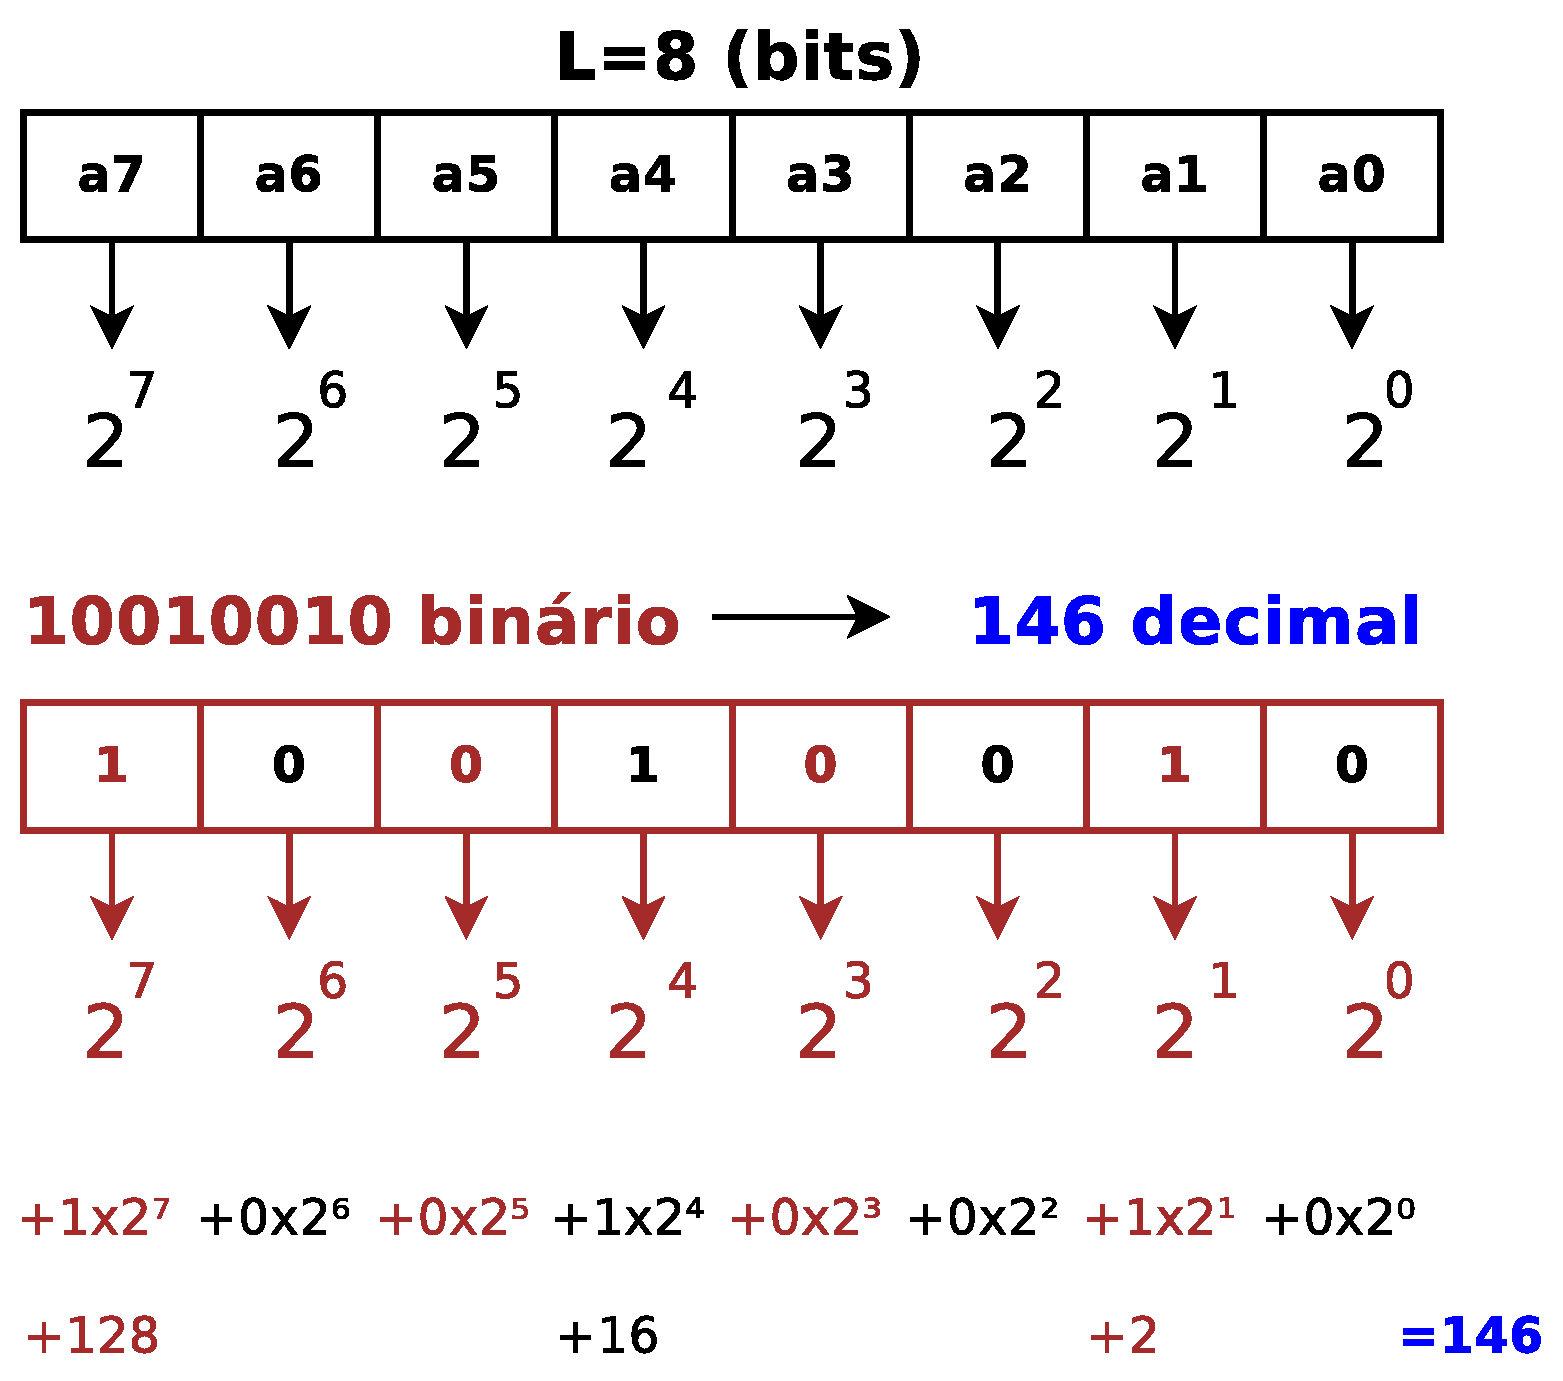
\includegraphics[width=1.0\textwidth]{images/binario2decimal.eps}
\end{center} 
\end{minipage}%
\begin{minipage}[c]{0.4\textwidth}
  \begin{equation}
A=\sum\limits_{i=0}^{L-1}{a_{i}2^i}
  \end{equation}
\end{minipage}
\end{frame}

%%%%%%%%%%%%%%%%%%%%%%%%%%%%%%%%%%%%%%%%%%%%%%%%%%%%%%%%%%%%%%%%%%%%%%%%%%%%%%%%%
\begin{frame}{Soma de números inteiros positivos}
\begin{minipage}[c]{0.5\textwidth}
\begin{center}
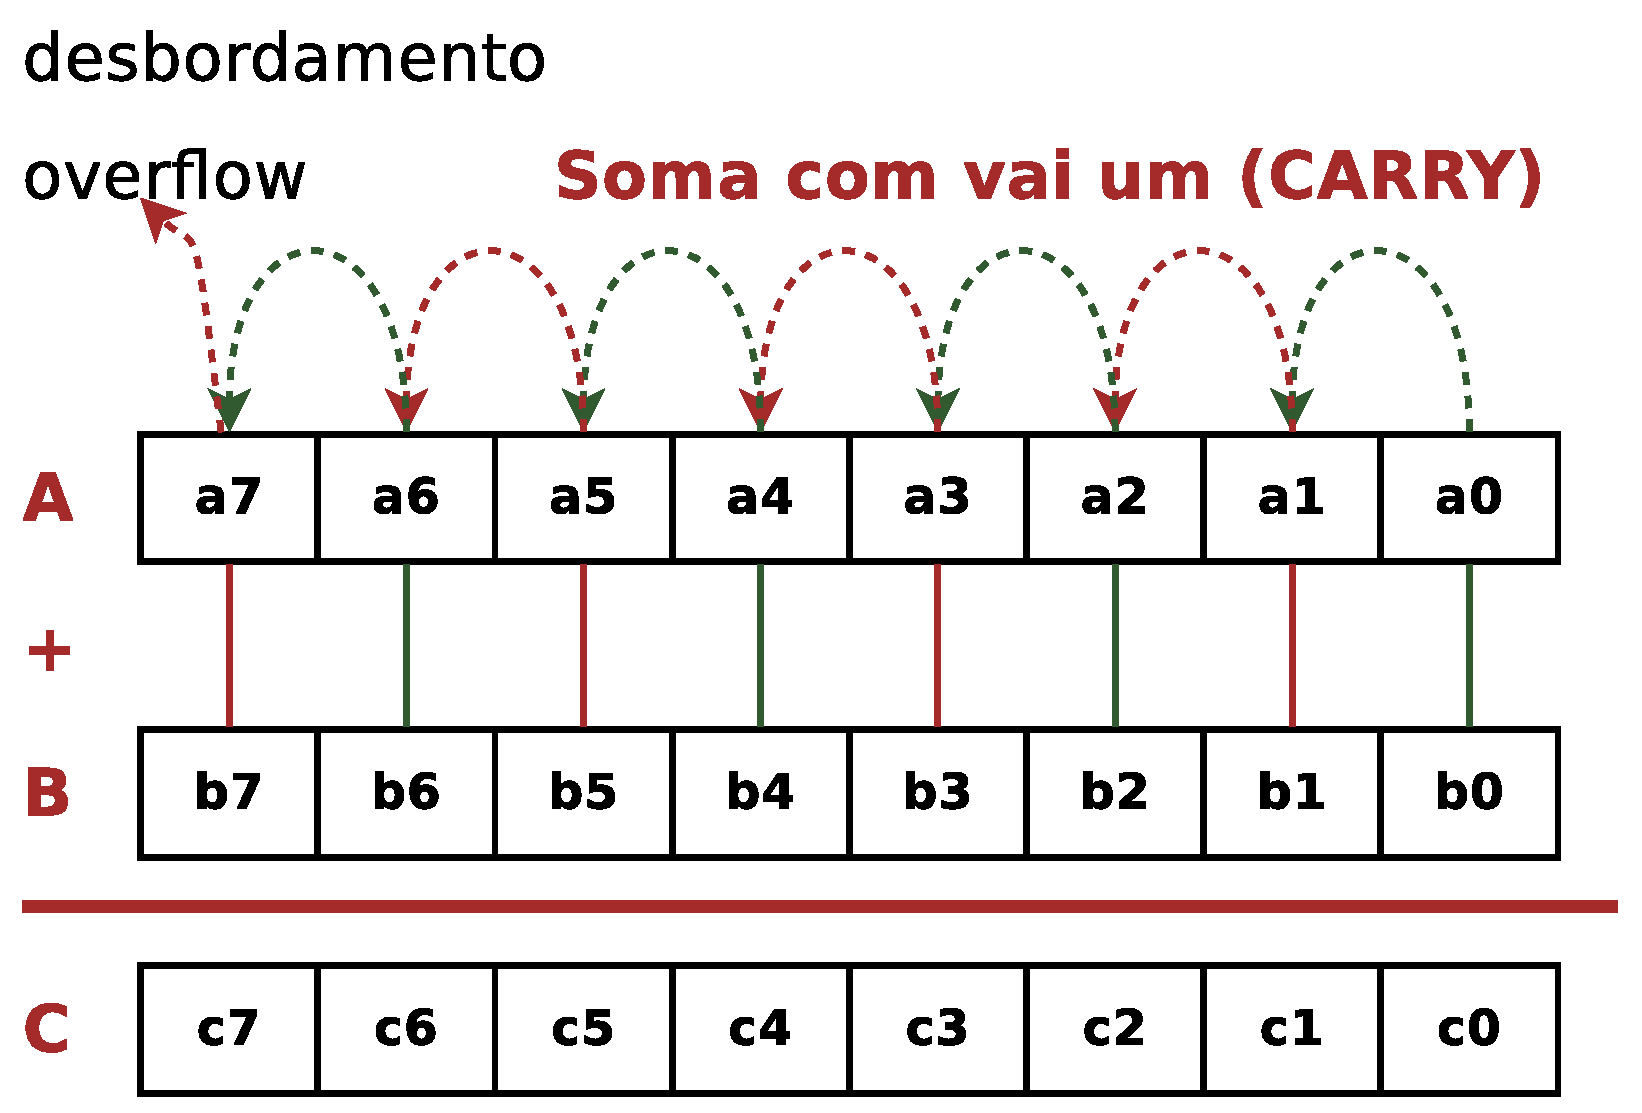
\includegraphics[width=1.0\textwidth]{images/somainteira1.eps}
\end{center} 
\end{minipage}%
\begin{minipage}[c]{0.5\textwidth}
\begin{center}
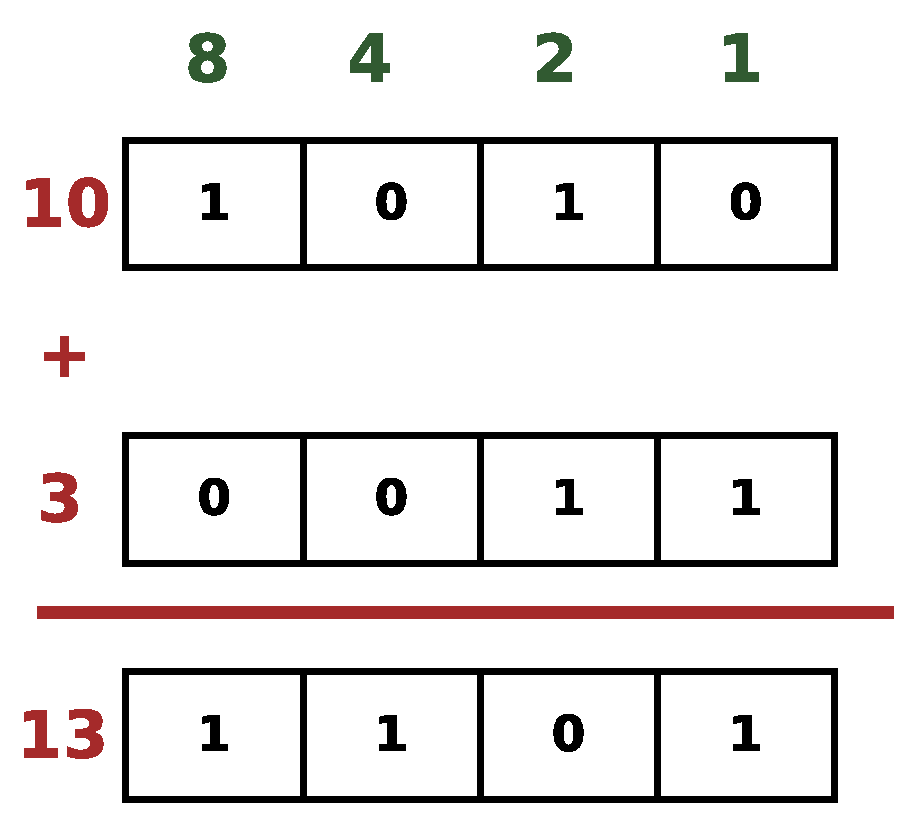
\includegraphics[width=1.0\textwidth]{images/somainteira2.eps}
\end{center} 
\end{minipage}
\end{frame}

%%%%%%%%%%%%%%%%%%%%%%%%%%%%%%%%%%%%%%%%%%%%%%%%%%%%%%%%%%%%%%%%%%%%%%%%%%%%%%%%%
\begin{frame}{Soma de números inteiros positivos (desboradmento)}
\begin{minipage}[c]{0.5\textwidth}
\begin{center}
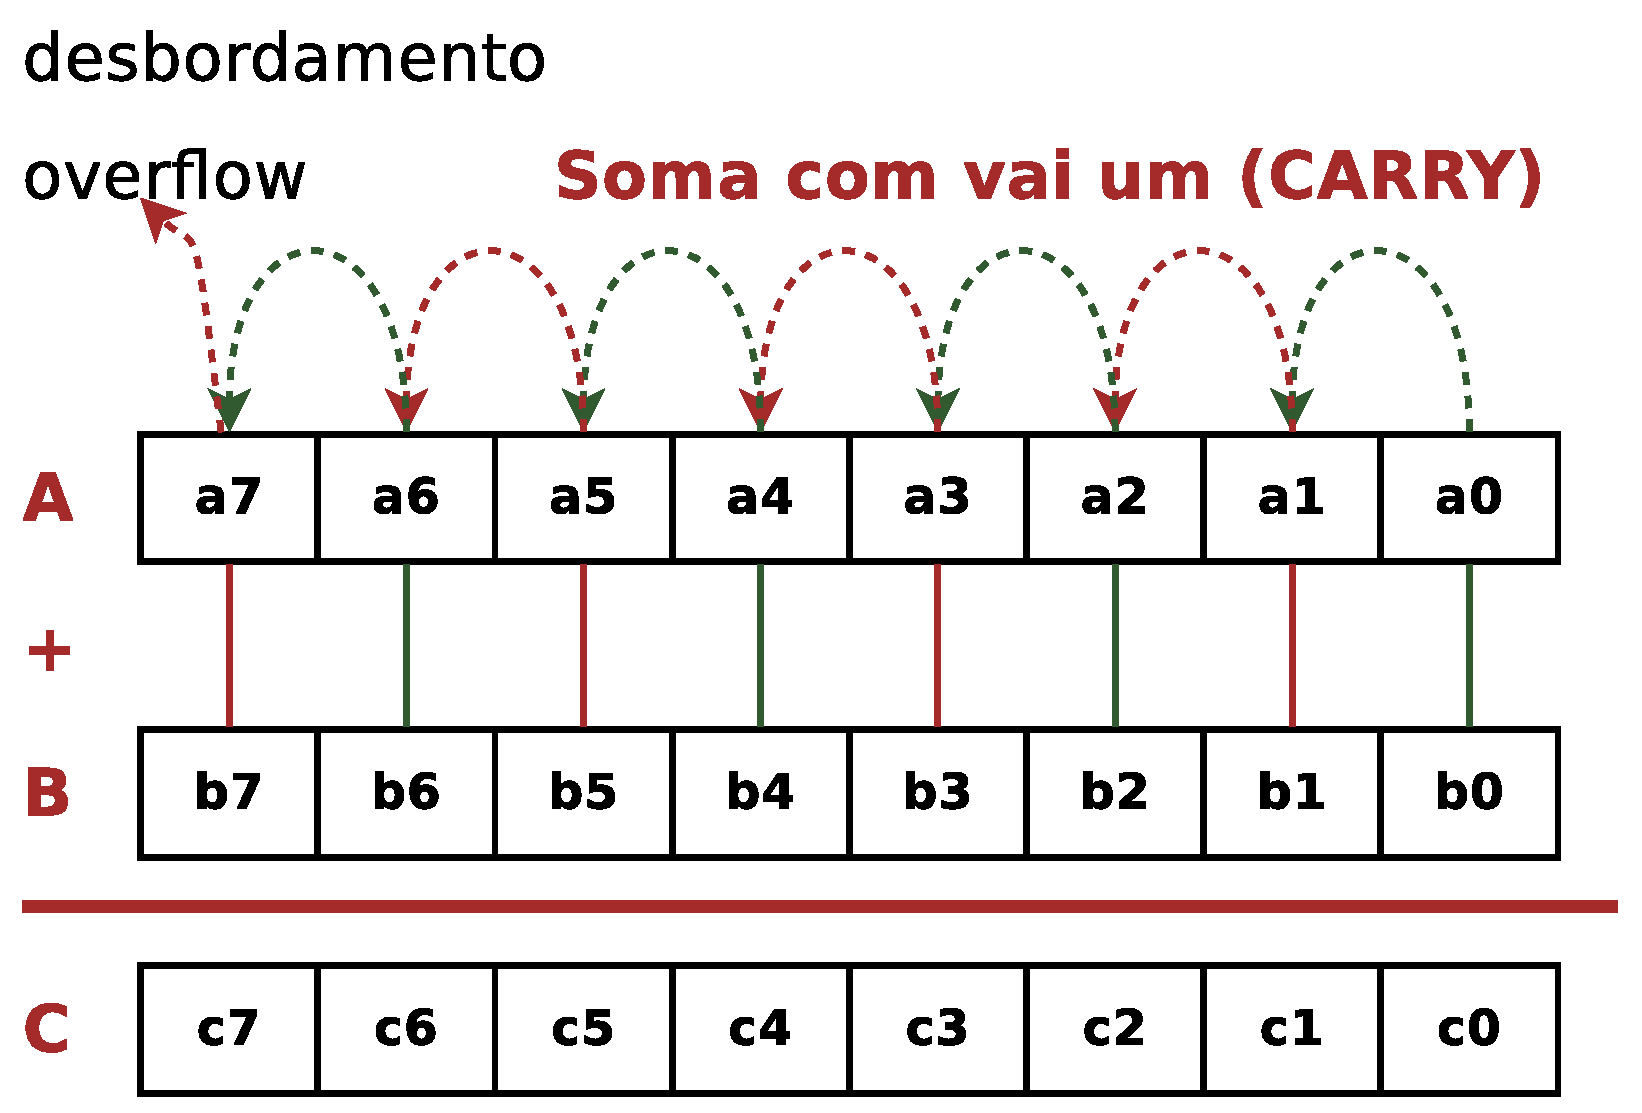
\includegraphics[width=1.0\textwidth]{images/somainteira1.eps}
\end{center} 
\end{minipage}%
\begin{minipage}[c]{0.5\textwidth}
\begin{center}
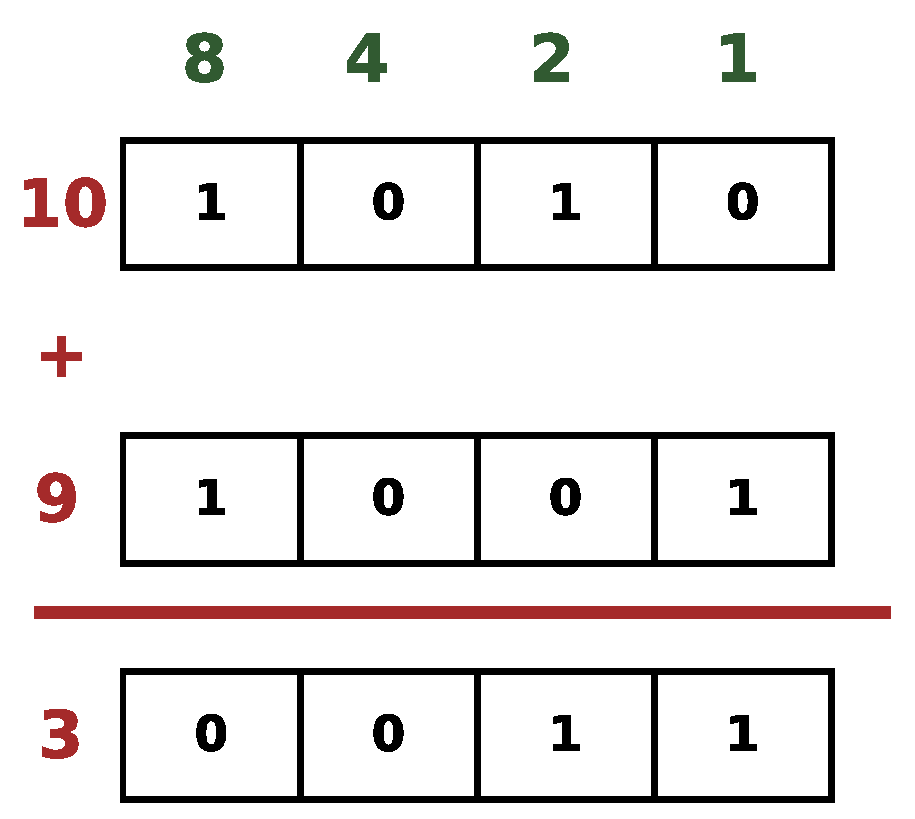
\includegraphics[width=1.0\textwidth]{images/somainteira3.eps}
\end{center} 
\end{minipage}
\end{frame}

%%%%%%%%%%%%%%%%%%%%%%%%%%%%%%%%%%%%%%%%%%%%%%%%%%%%%%%%%%%%%%%%%%%%%%%%%%%%%%%%%
\begin{frame}{Multiplicação de números inteiros positivos}
\begin{center}
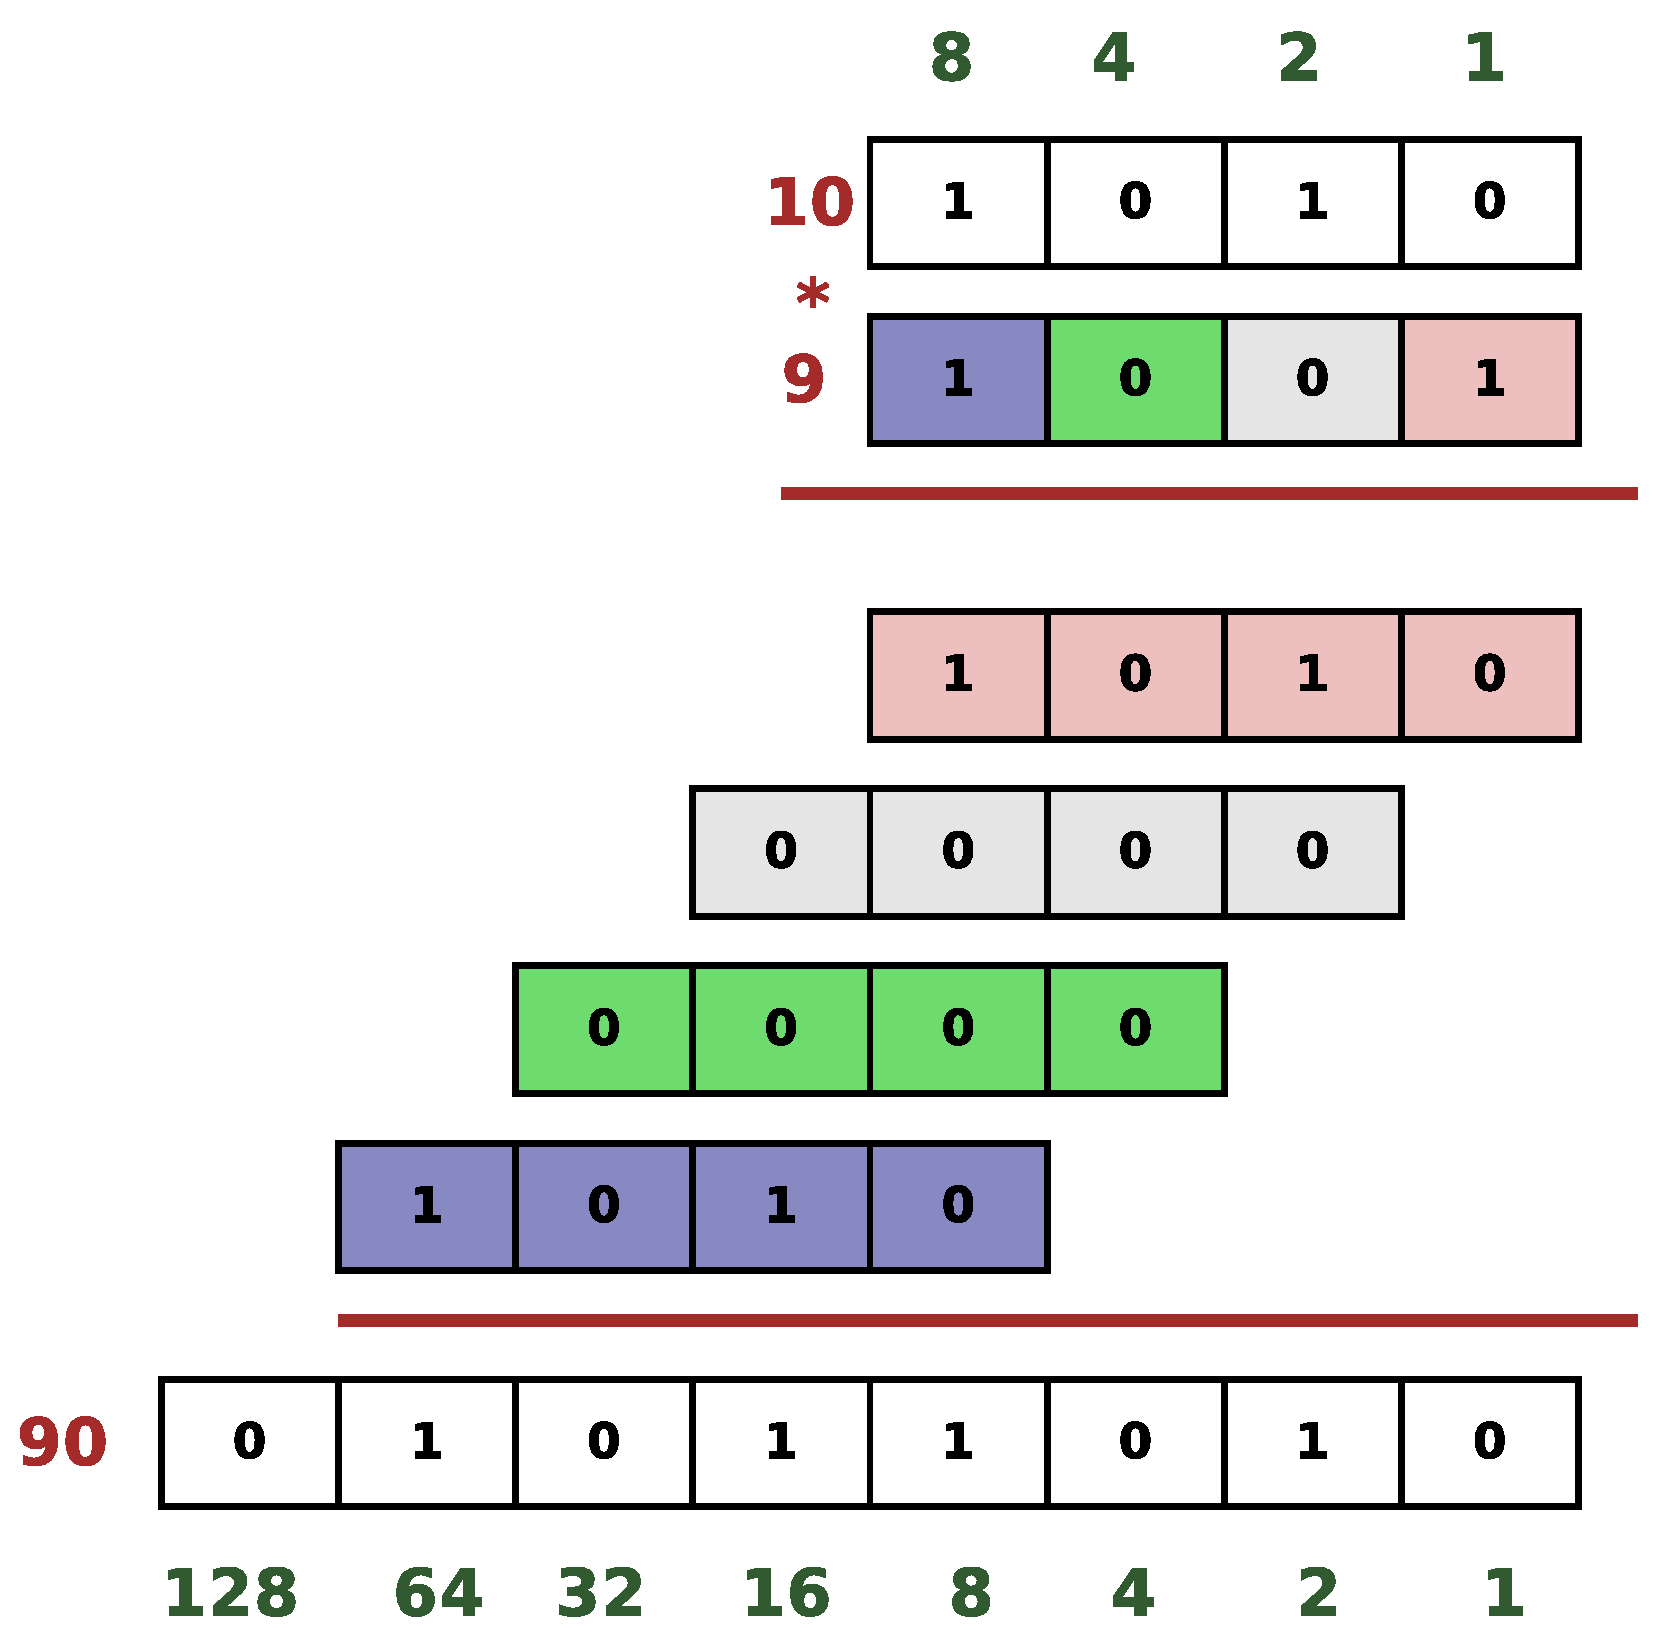
\includegraphics[width=0.5\textwidth]{images/mulinteira2.eps}
\end{center} 
\end{frame}

%%%%%%%%%%%%%%%%%%%%%%%%%%%%%%%%%%%%%%%%%%%%%%%%%%%%%%%%%%%%%%%%%%%%%%%%%%%%%%%%%
\begin{frame}{Multiplicação de números inteiros positivos}
\begin{center}
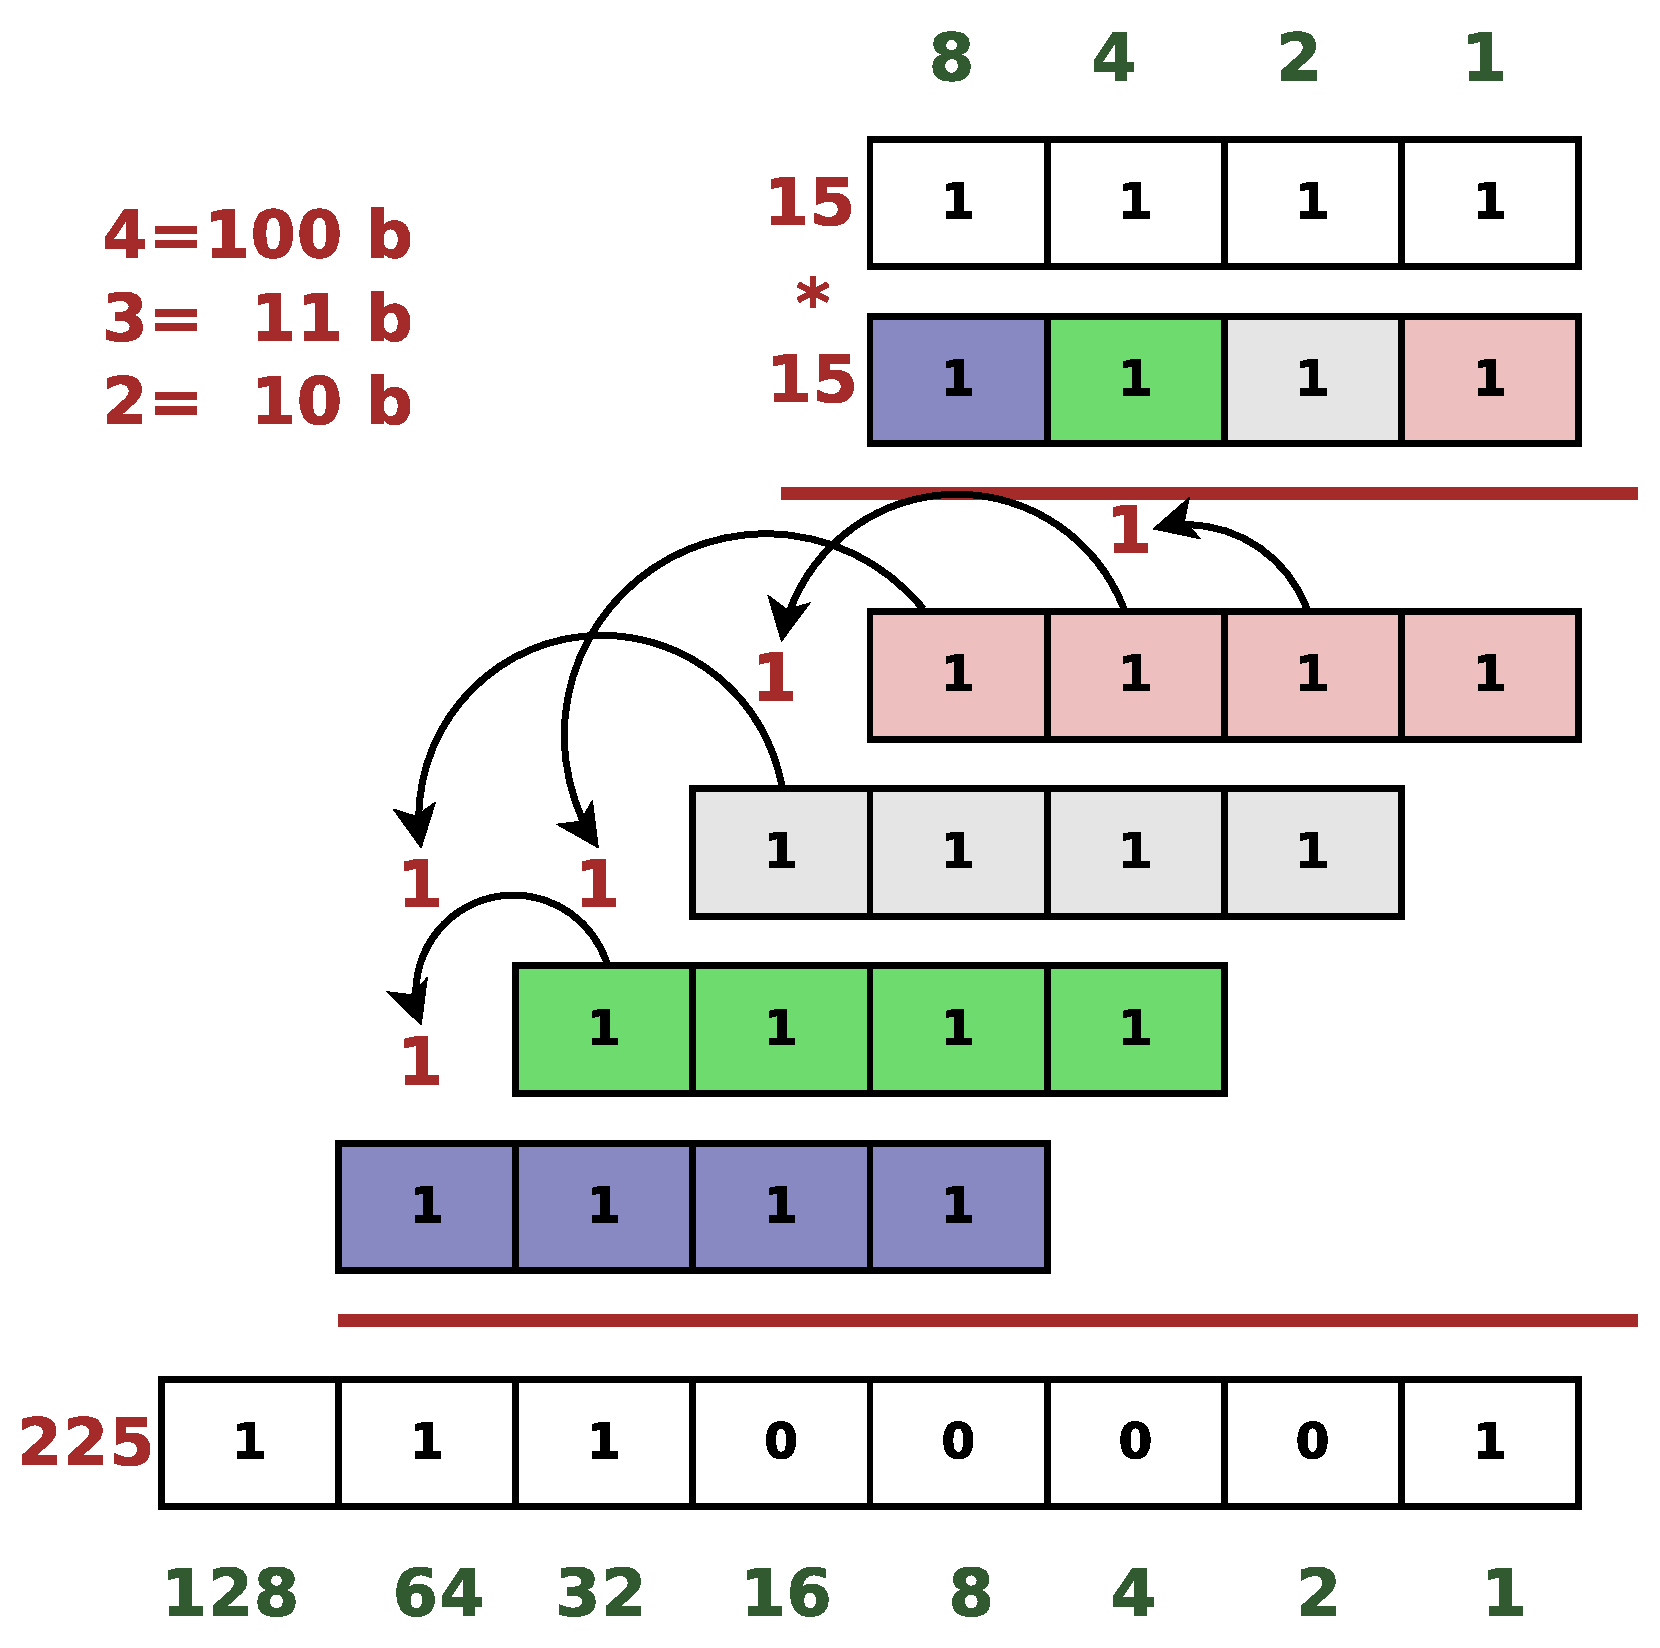
\includegraphics[width=0.5\textwidth]{images/mulinteira3.eps}
\end{center} 
\end{frame}

%%%%%%%%%%%%%%%%%%%%%%%%%%%%%%%%%%%%%%%%%%%%%%%%%%%%%%%%%%%%%%%%%%%%%%%%%%%%%%%%%
\begin{frame}{Divisão de números inteiros positivos}
\begin{center}
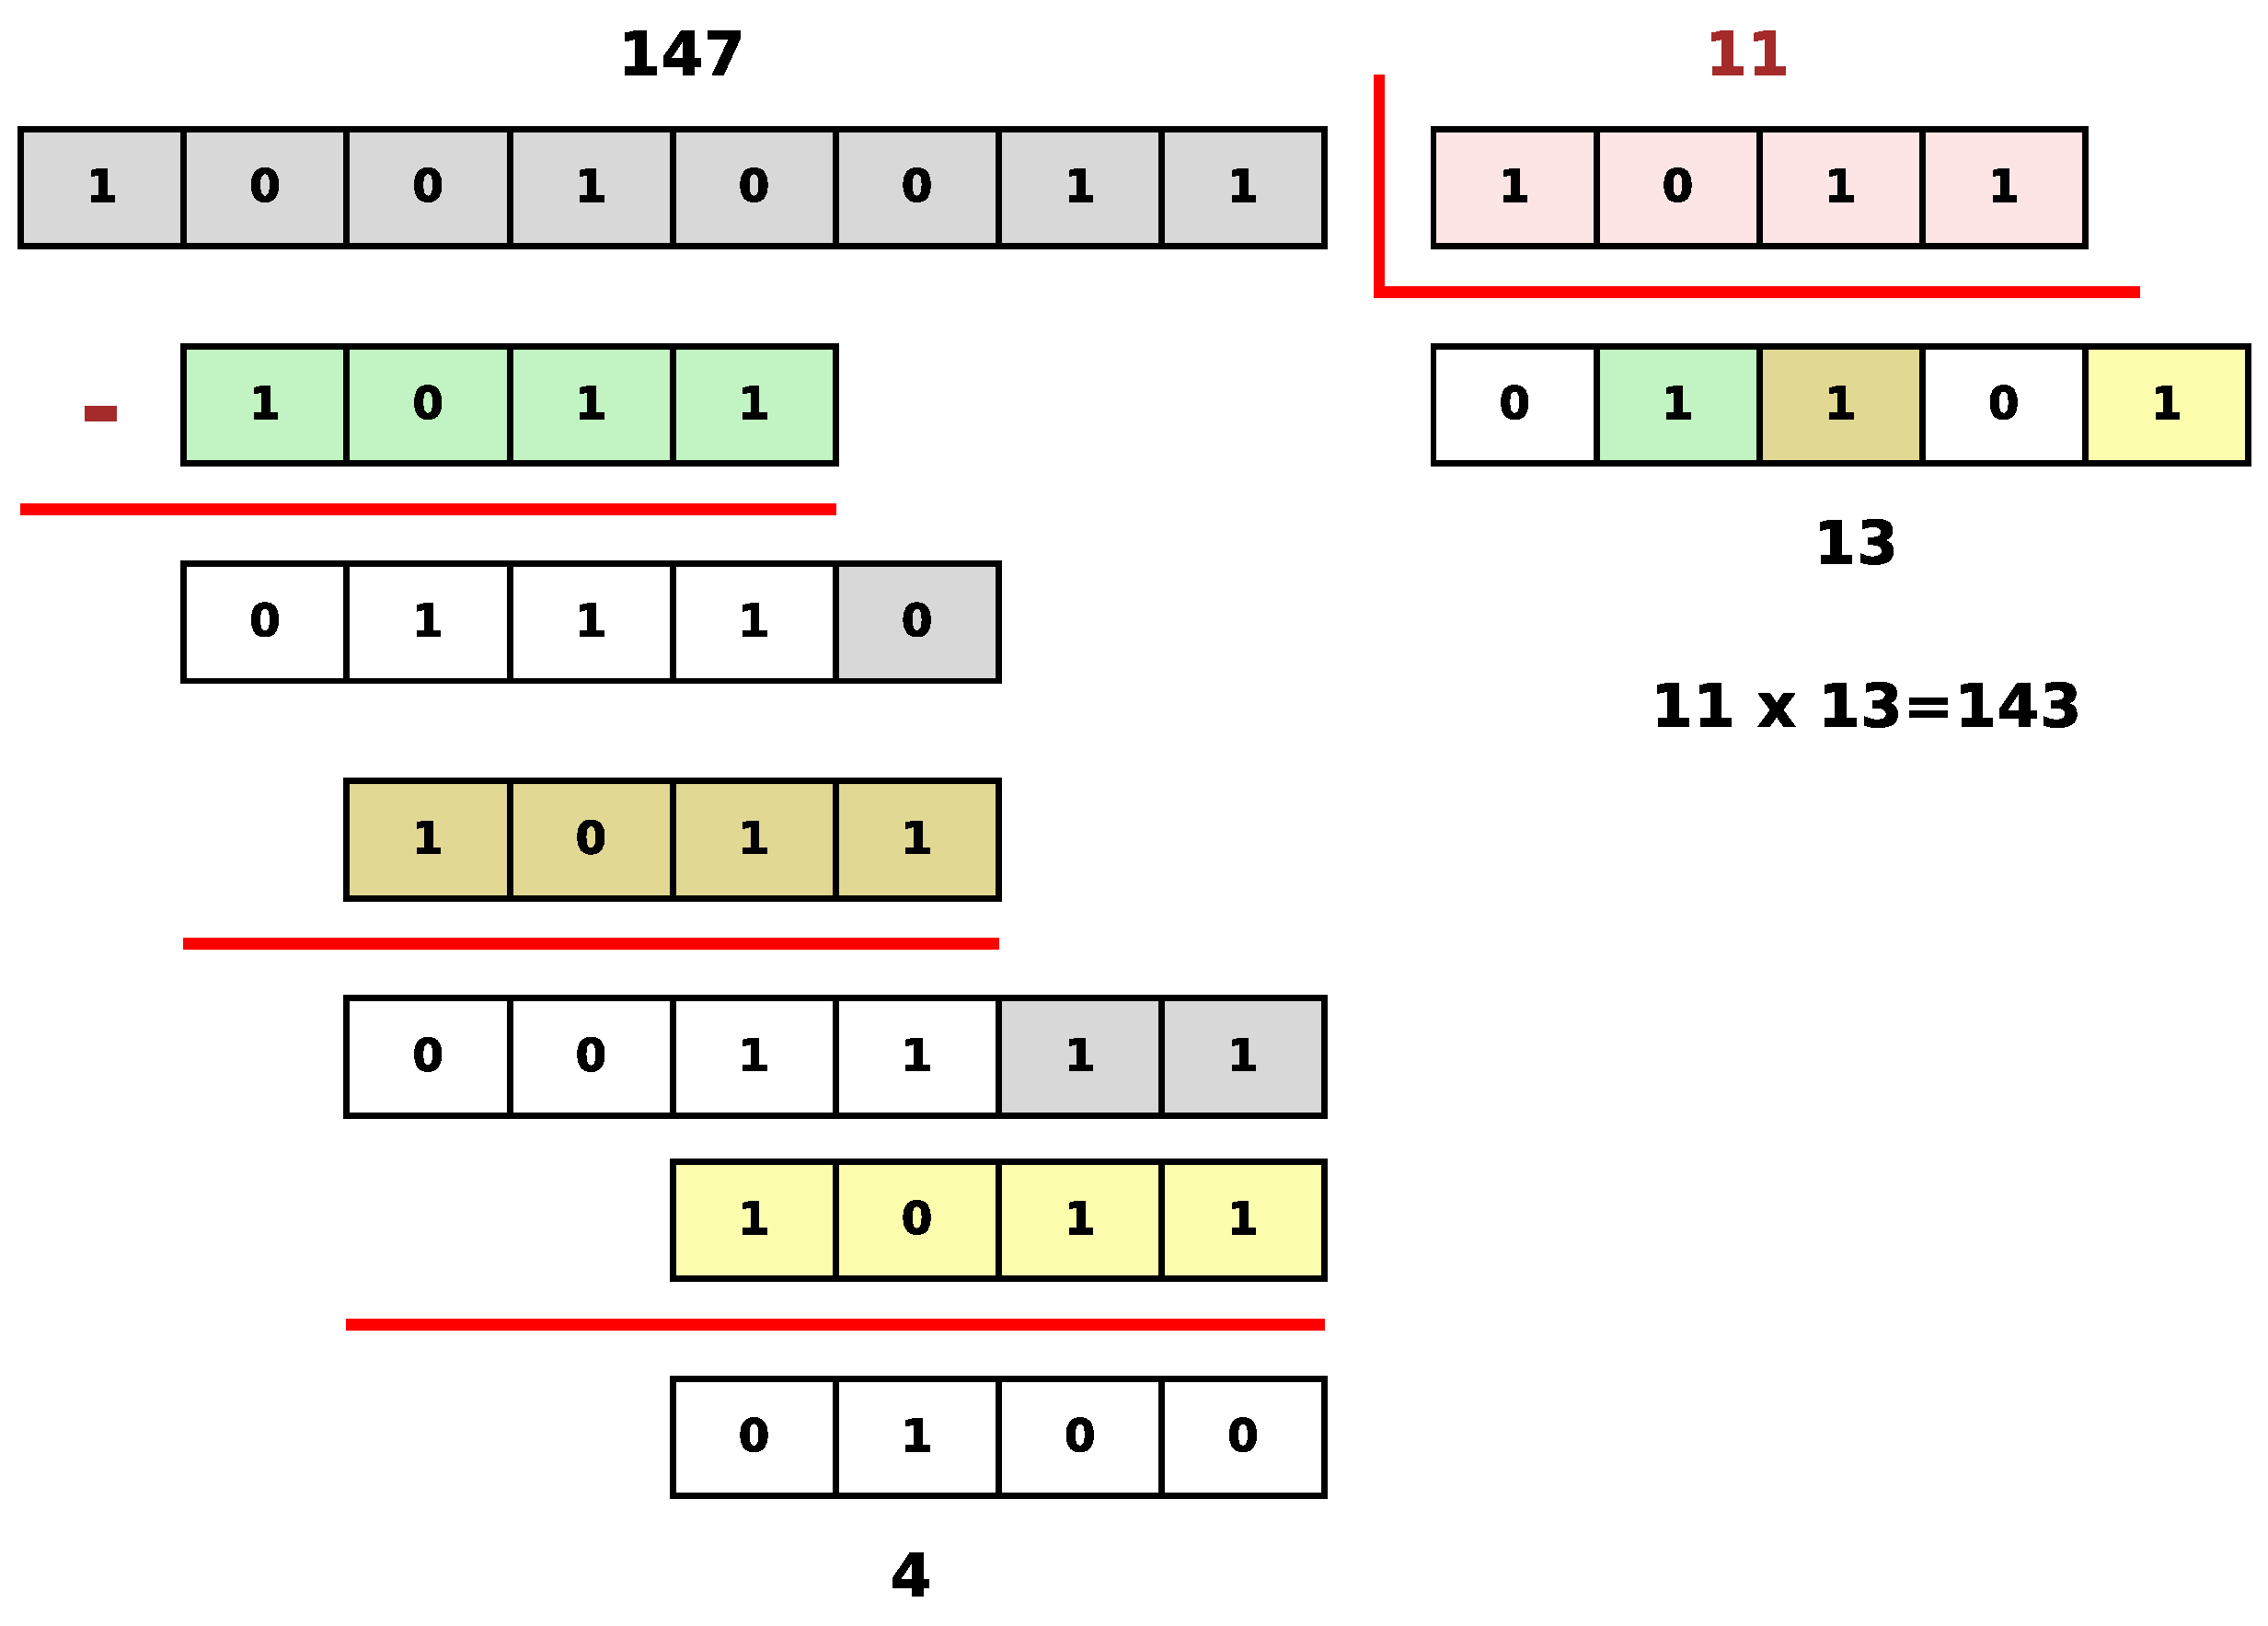
\includegraphics[width=0.7\textwidth]{images/divide.eps}
\end{center} 
\end{frame}

%%%%%%%%%%%%%%%%%%%%%%%%%%%%%%%%%%%%%%%%%%%%%%%%%%%%%%%%%%%%%%%%%%%%%%%%%%%%%%%%
%%%%%%%%%%%%%%%%%%%%%%%%%%%%%%%%%%%%%%%%%%%%%%%%%%%%%%%%%%%%%%%%%%%%%%%%%%%%%%%%
\section{Aritmética com inteiros negativos}
%%%%%%%%%%%%%%%%%%%%%%%%%%%%%%%%%%%%%%%%%%%%%%%%%%%%%%%%%%%%%%%%%%%%%%%%%%%%%%%%%
\begin{frame}{Num. negativo com representação Sinal-magnitude \cite{arq}}
00000000=0~dec~~???~~10000000=0~dec
\begin{minipage}[c]{0.5\textwidth}
~\\
\begin{center}
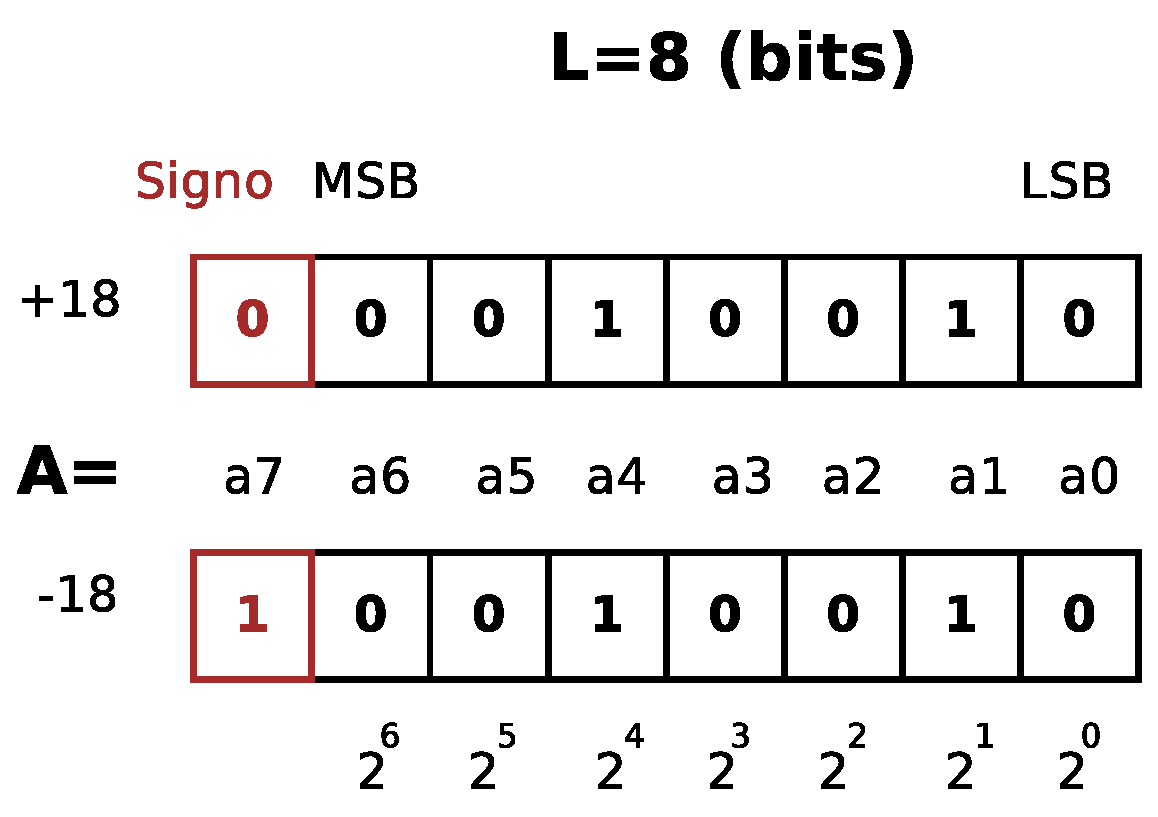
\includegraphics[width=1.0\textwidth]{images/sinalmag.eps}
\end{center} 
~\\
~\\
\end{minipage}%
\begin{minipage}[c]{0.5\textwidth}
  \begin{equation}
D_A=\begin{cases}
 +\sum\limits_{i=0}^{L-2}{a_{i}2^i} & \text{ if } a_{L-1}=0 \\ 
 ~ & ~\\
 -\sum\limits_{i=0}^{L-2}{a_{i}2^i} & \text{ if } a_{L-1}=1 
\end{cases}
  \end{equation}
\end{minipage}
\end{frame}
%%%%%%%%%%%%%%%%%%%%%%%%%%%%%%%%%%%%%%%%%%%%%%%%%%%%%%%%%%%%%%%%%%%%%%%%%%%%%%%%%
\begin{frame}{Num. negativo com representação complemento a dois}
~~{\color{red}$X=\overline{A}+1$},~~~~~~{\color{red}$X$ é o complemento a dois de $A$}.\\
$-A=\overline{A}+1$,~~~~$-A$ é o complemento a dois de $A$.
\begin{minipage}[c]{0.5\textwidth}
\begin{center}
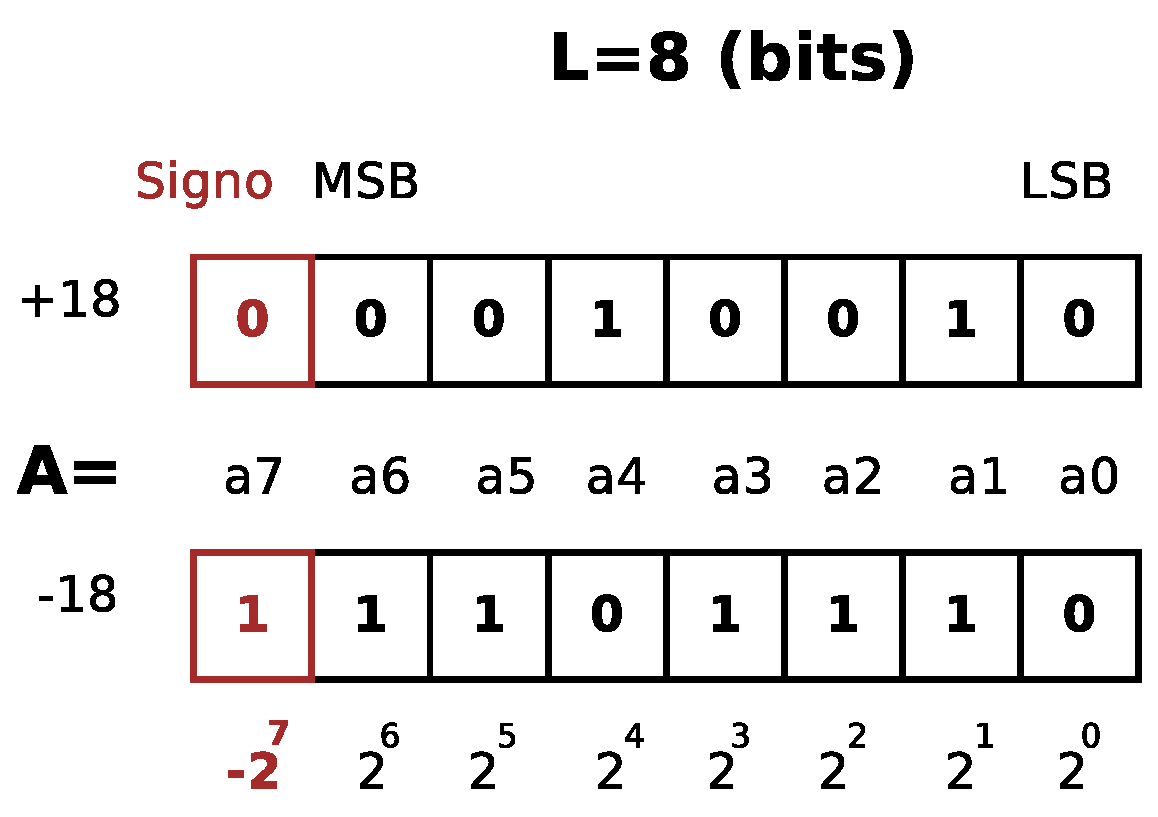
\includegraphics[width=1.0\textwidth]{images/complementoadois0.eps}
\end{center} 
\end{minipage}%
\begin{minipage}[c]{0.5\textwidth}
  \begin{equation}
D_A=-2^{L-1}a_{L-1}+\sum\limits_{i=0}^{L-2}{a_{i}2^i}
  \end{equation}
\end{minipage}
\end{frame}
%%%%%%%%%%%%%%%%%%%%%%%%%%%%%%%%%%%%%%%%%%%%%%%%%%%%%%%%%%%%%%%%%%%%%%%%%%%%%%%%%
\begin{frame}{Num. negativo com representação complemento a dois}
~~{\color{red}$X=\overline{A}+1$},~~~~~~{\color{red}$X$ é o complemento a dois de $A$}.\\
$-A=\overline{A}+1$,~~~~$-A$ é o complemento a dois de $A$.
\begin{minipage}[c]{0.5\textwidth}
\begin{center}
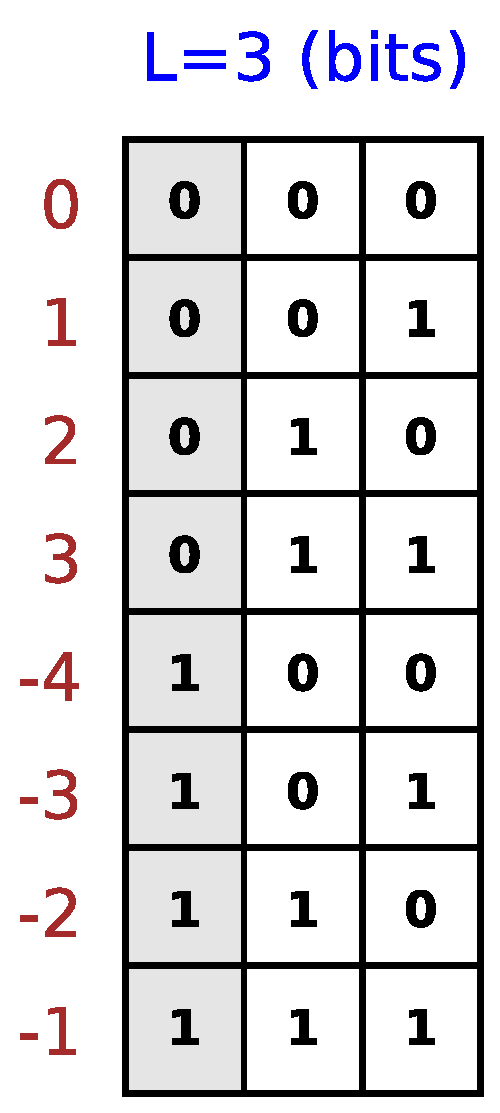
\includegraphics[width=0.4\textwidth]{images/complementoadois1.eps}
\end{center} 
\end{minipage}%
\begin{minipage}[c]{0.5\textwidth}
  \begin{equation}
-2^{L-1} \leq A \leq 2^{L-1}-1
  \end{equation}
  \begin{equation}
B-A=B+\overline{A}+1
  \end{equation}
\end{minipage}
\end{frame}
%%%%%%%%%%%%%%%%%%%%%%%%%%%%%%%%%%%%%%%%%%%%%%%%%%%%%%%%%%%%%%%%%%%%%%%%%%%%%%%%%
\begin{frame}{Soma de números inteiros em complemento a dois}
\begin{minipage}[c]{0.5\textwidth}
\begin{center}
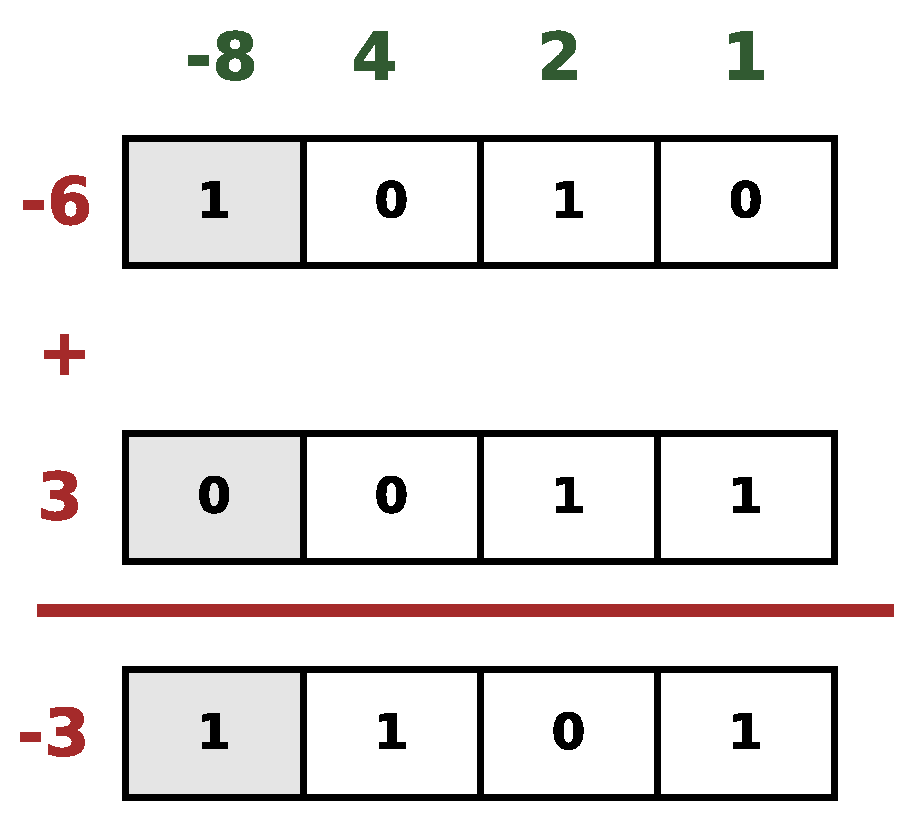
\includegraphics[width=0.9\textwidth]{images/somainteirac2a.eps}
\end{center} 
\end{minipage}%
\begin{minipage}[c]{0.5\textwidth}
\begin{center}
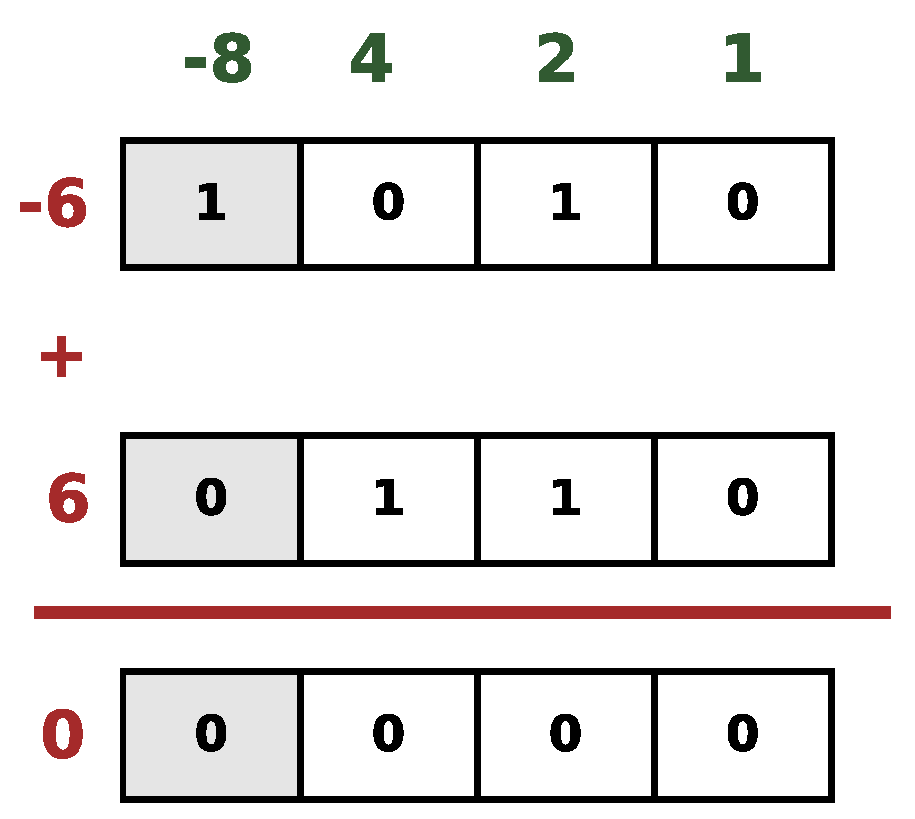
\includegraphics[width=0.9\textwidth]{images/somainteirac2b.eps}
\end{center} 
\end{minipage}
\end{frame}

%%%%%%%%%%%%%%%%%%%%%%%%%%%%%%%%%%%%%%%%%%%%%%%%%%%%%%%%%%%%%%%%%%%%%%%%%%%%%%%%%
\begin{frame}{Multiplicação de números inteiros em complemento a dois}
\begin{minipage}[c]{0.5\textwidth}
\begin{center}
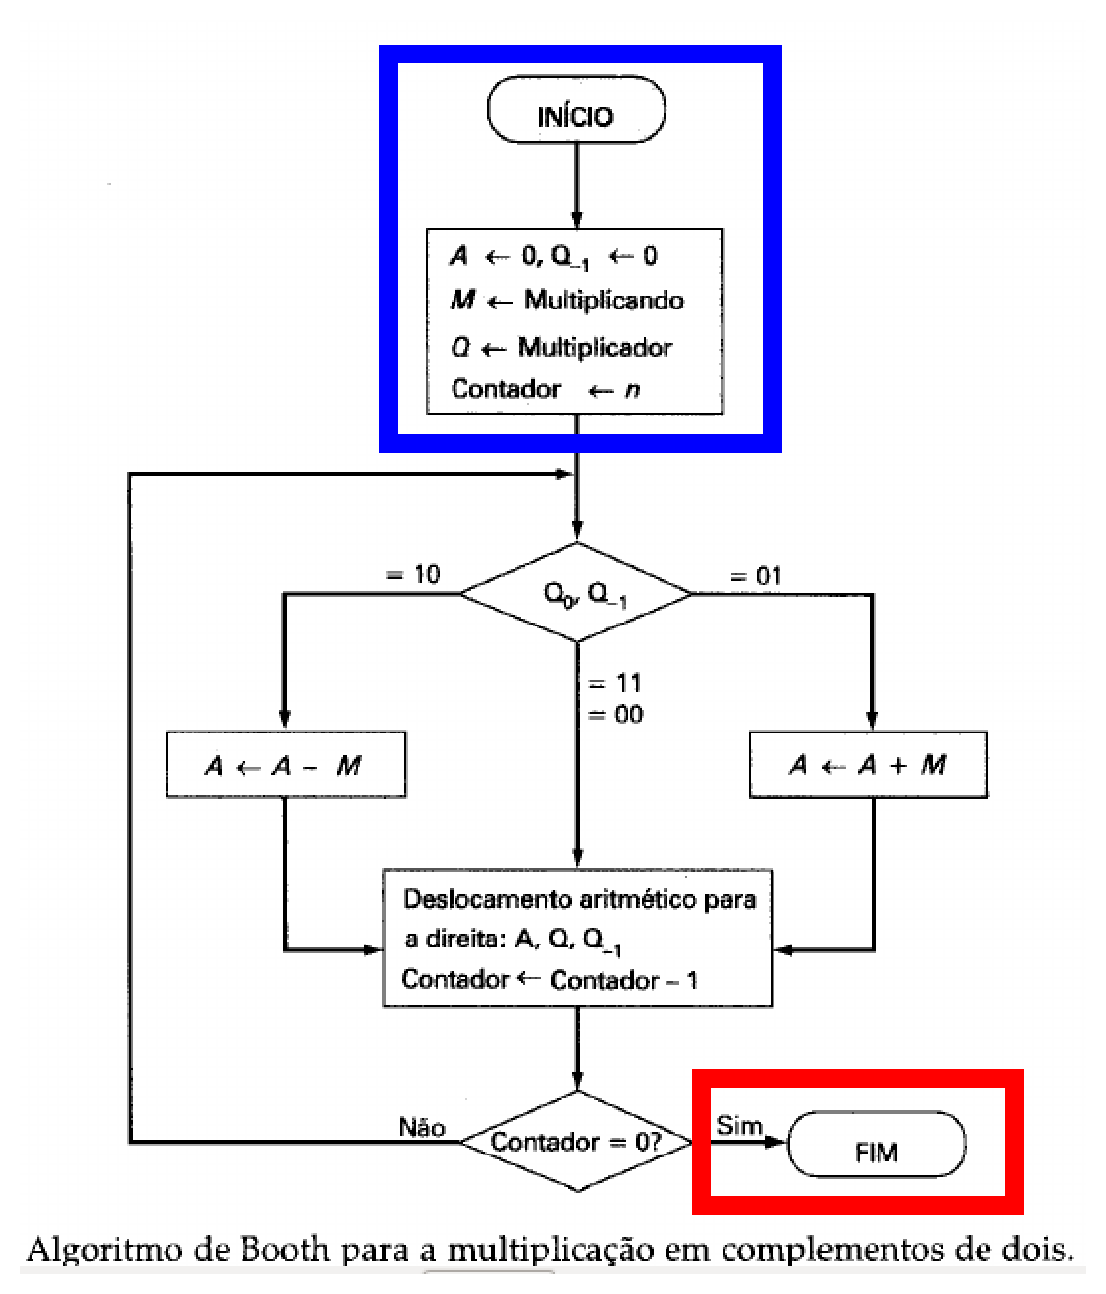
\includegraphics[width=1.0\textwidth]{images/booth.eps}
\end{center} 
\end{minipage}%
\begin{minipage}[c]{0.5\textwidth}
\begin{center}
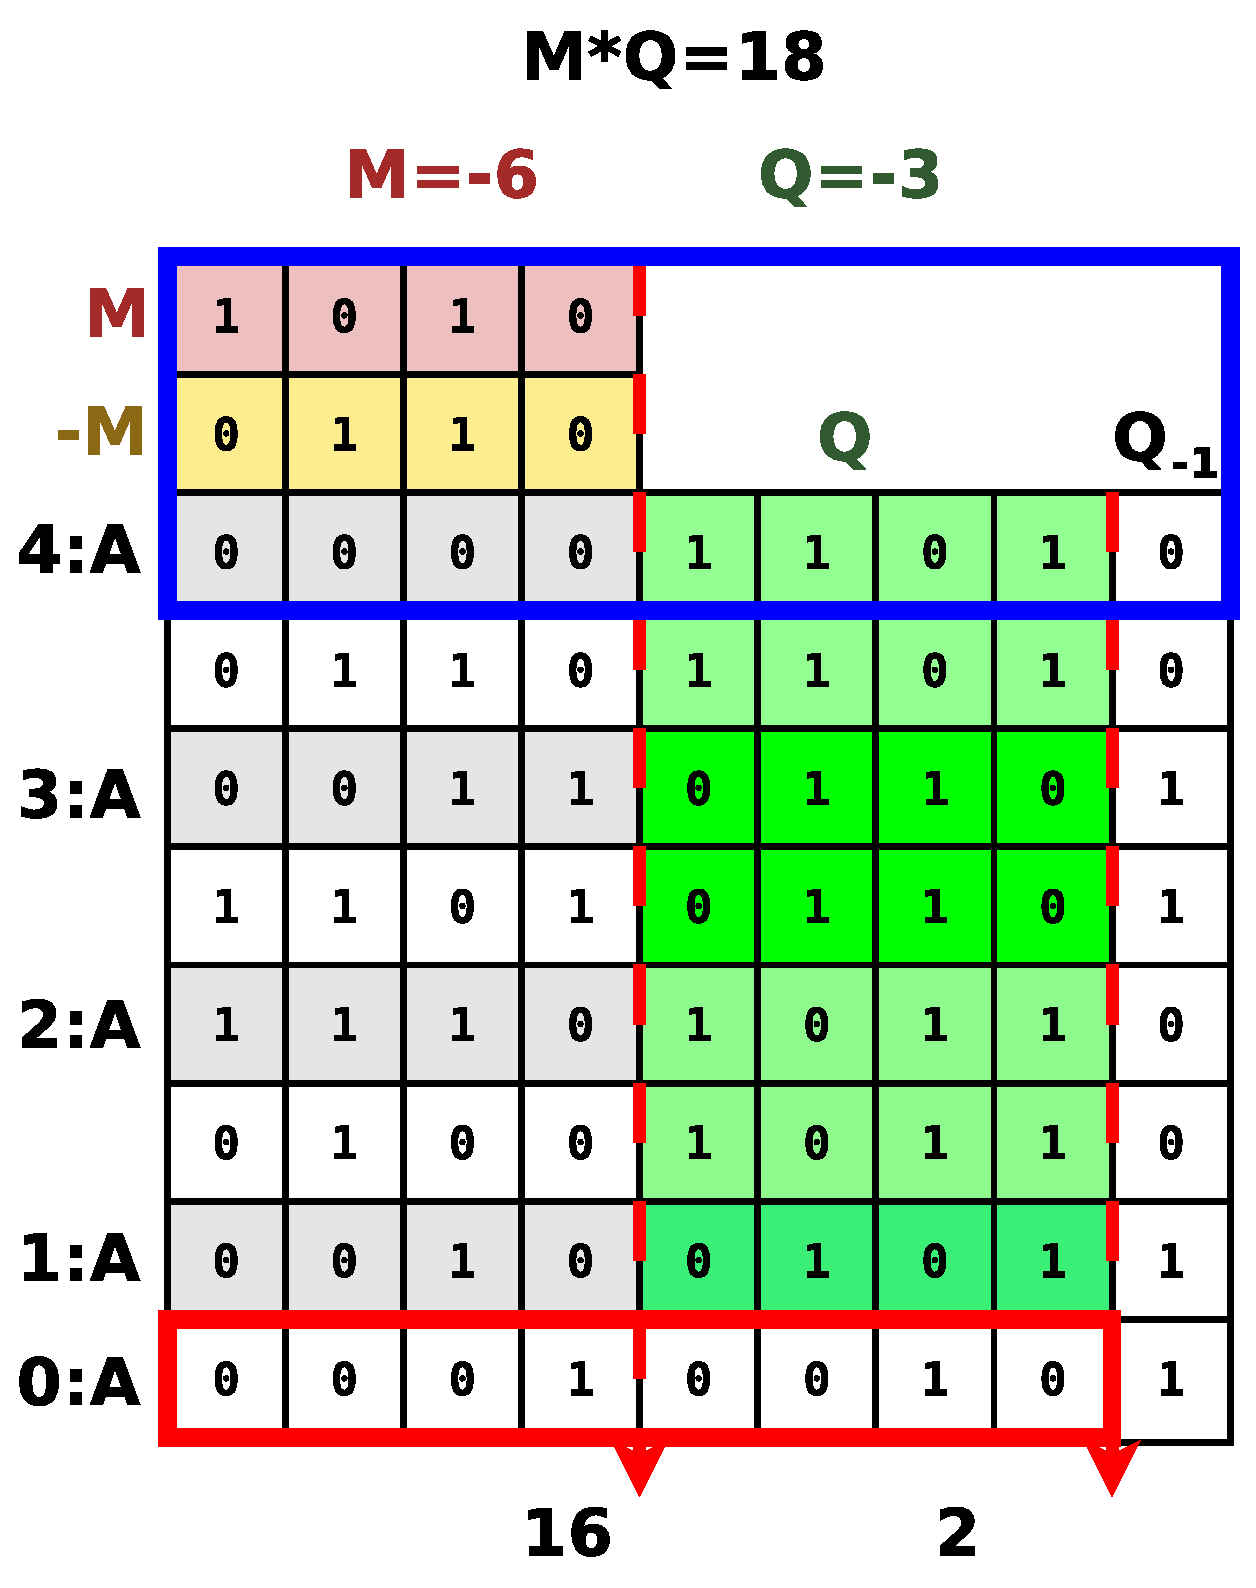
\includegraphics[width=0.9\textwidth]{images/booth2.eps}
\end{center} 
\end{minipage}
\end{frame}

%%%%%%%%%%%%%%%%%%%%%%%%%%%%%%%%%%%%%%%%%%%%%%%%%%%%%%%%%%%%%%%%%%%%%%%%%%%%%%%%%
\begin{frame}{Divisão de números inteiros com signo}
\begin{minipage}[c]{0.6\textwidth}
\begin{center}
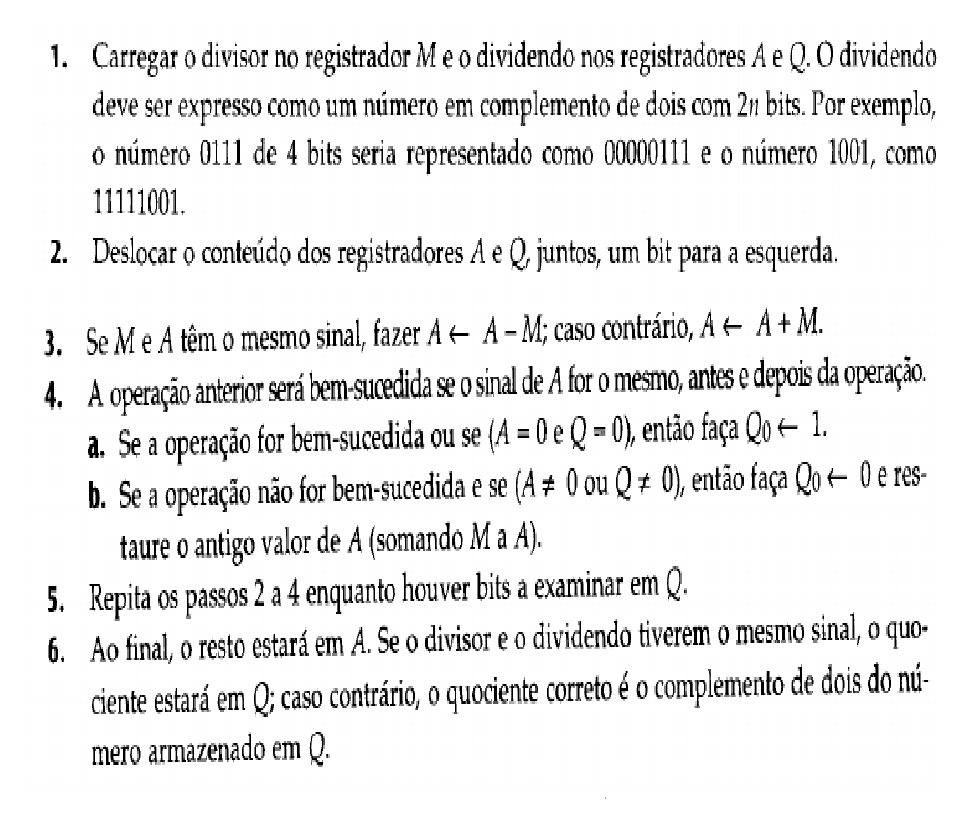
\includegraphics[width=1.0\textwidth]{images/dividesigno.eps}
\end{center}  
\end{minipage}%
\begin{minipage}[c]{0.4\textwidth}
\begin{center}
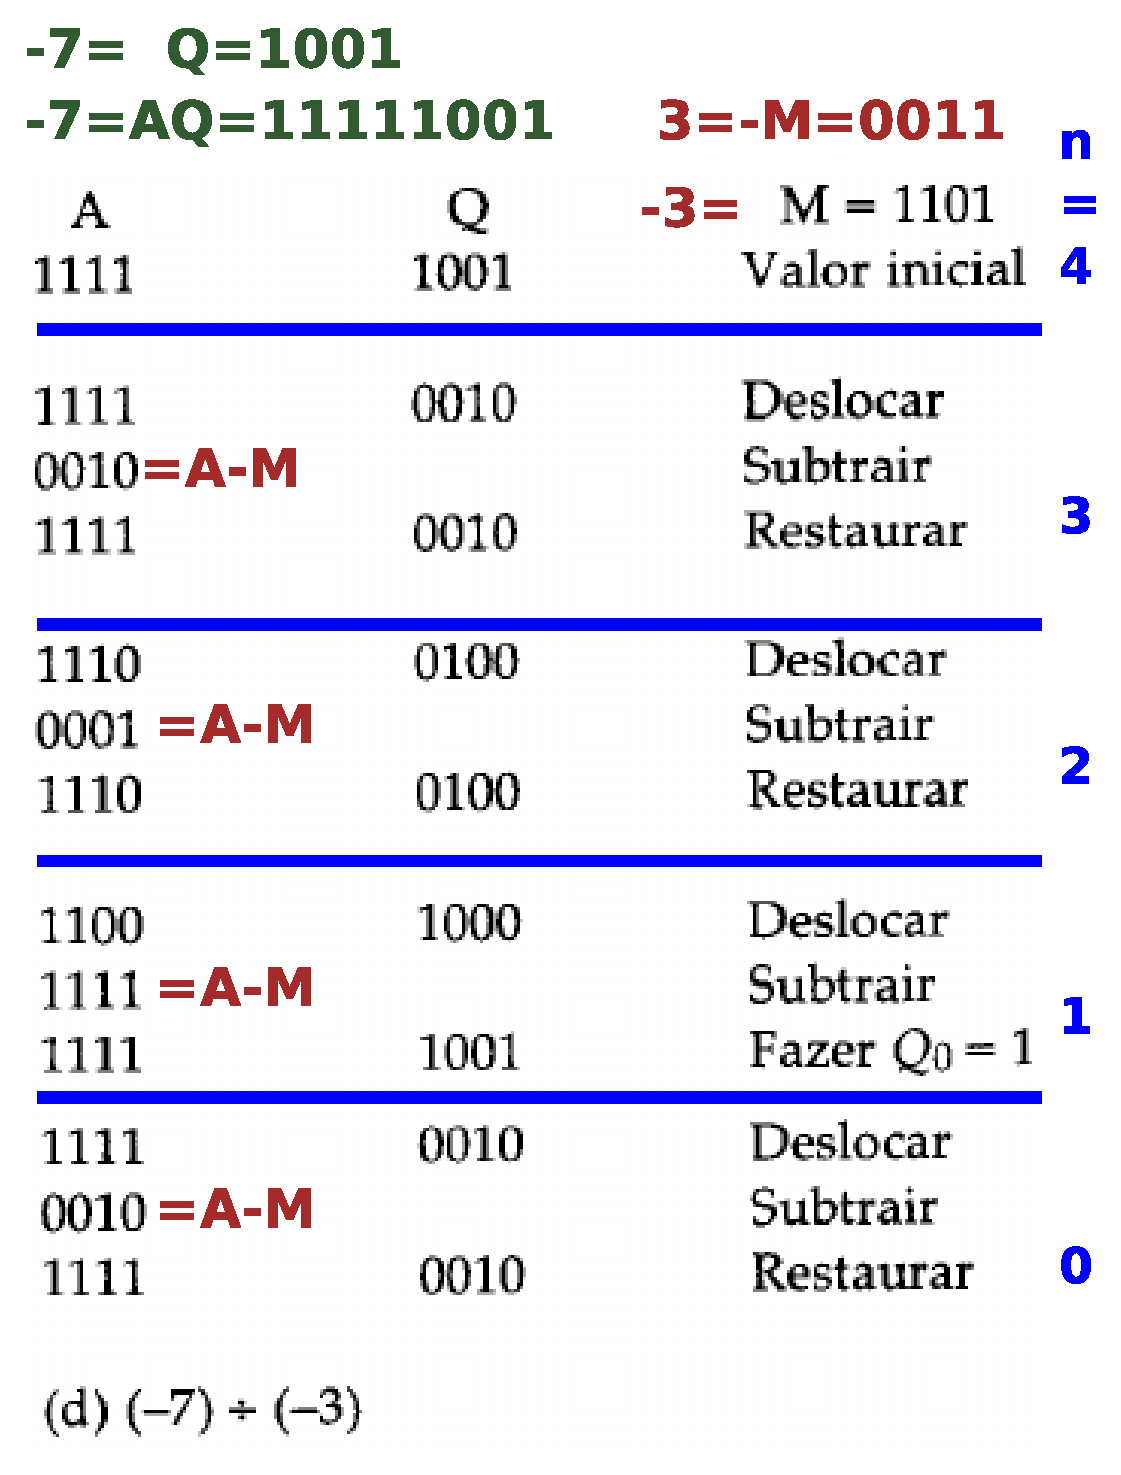
\includegraphics[width=1.0\textwidth]{images/dividesigno2.eps}
\end{center}  
\end{minipage}
\end{frame}
%%%%%%%%%%%%%%%%%%%%%%%%%%%%%%%%%%%%%%%%%%%%%%%%%%%%%%%%%%%%%%%%%%%%%%%%%%%%%%%%
%%%%%%%%%%%%%%%%%%%%%%%%%%%%%%%%%%%%%%%%%%%%%%%%%%%%%%%%%%%%%%%%%%%%%%%%%%%%%%%%
\section{Representação em ponto flutuante}
%%%%%%%%%%%%%%%%%%%%%%%%%%%%%%%%%%%%%%%%%%%%%%%%%%%%%%%%%%%%%%%%%%%%%%%%%%%%%%%%%
\begin{frame}{Representação em ponto flutuante \cite{arq}}
\begin{minipage}[c]{0.5\textwidth}
\begin{center}
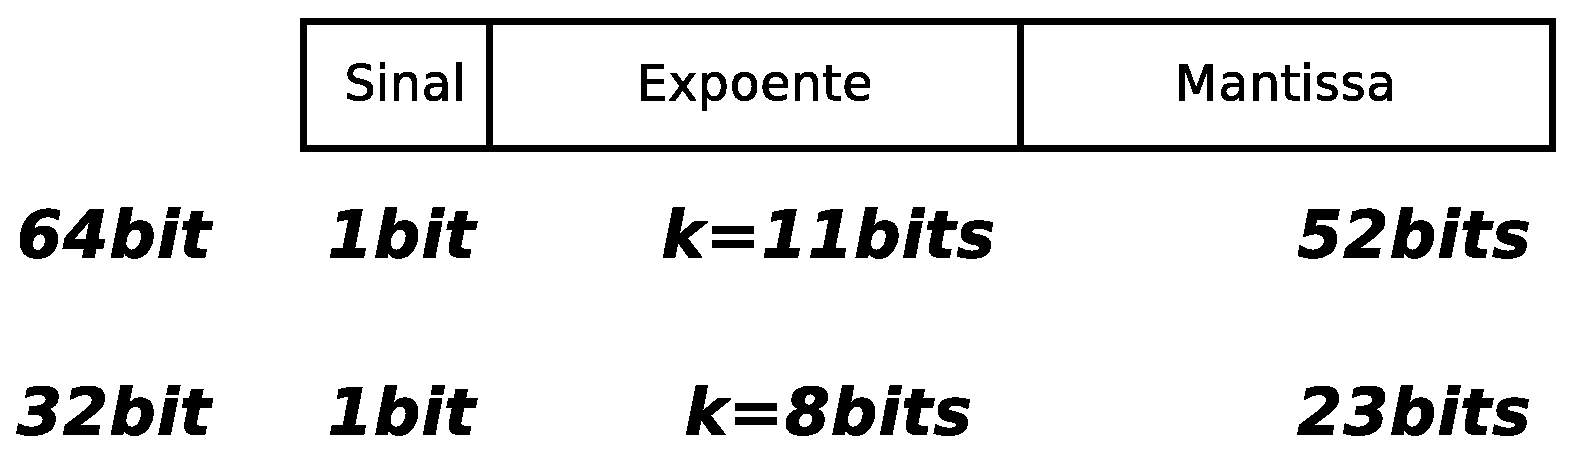
\includegraphics[width=0.9\textwidth]{images/flutuante.eps}
\end{center}
\begin{varblock}{IEEE-754}
{\color{red}\begin{equation*}
s~1.M~2^E 
\end{equation*}}%
\begin{equation*}
s \equiv \begin{cases}
+&~~se~~Sinal\equiv0\\
-&~~se~~Sinal\equiv1
    \end{cases}
\end{equation*}
\begin{equation*}
 M \equiv Mantissa
\end{equation*}
\begin{equation*}
 E \equiv Expoente - \left( 2^{k-1}-1\right)
\end{equation*}
\end{varblock}
\end{minipage}%
\begin{minipage}[c]{0.5\textwidth}
\begin{varblock}{IEEE-754}
\begin{center}
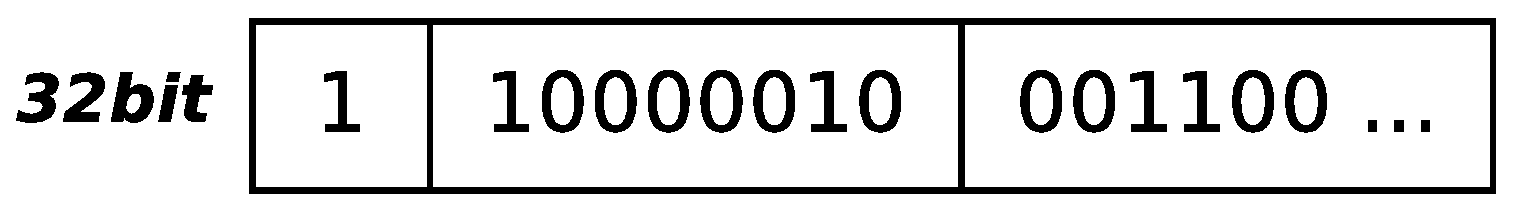
\includegraphics[width=1.0\textwidth]{images/flutuante2.eps}
\end{center}
\begin{equation*}
 S \equiv -
\end{equation*}
\begin{equation*}
 M \equiv 00110000...
\end{equation*}
\begin{equation*}
 E \equiv 130 - 127 = 3
\end{equation*}
{\color{red}
\begin{equation*}
-~1.0011~2^3 
\end{equation*}
\begin{equation*}
-~9.5
\end{equation*}}
\end{varblock}
\end{minipage}
\end{frame}

%%%%%%%%%%%%%%%%%%%%%%%%%%%%%%%%%%%%%%%%%%%%%%%%%%%%%%%%%%%%%%%%%%%%%%%%%%%%%%%%%
\begin{frame}{Divisão de números inteiros positivos}
\begin{center}
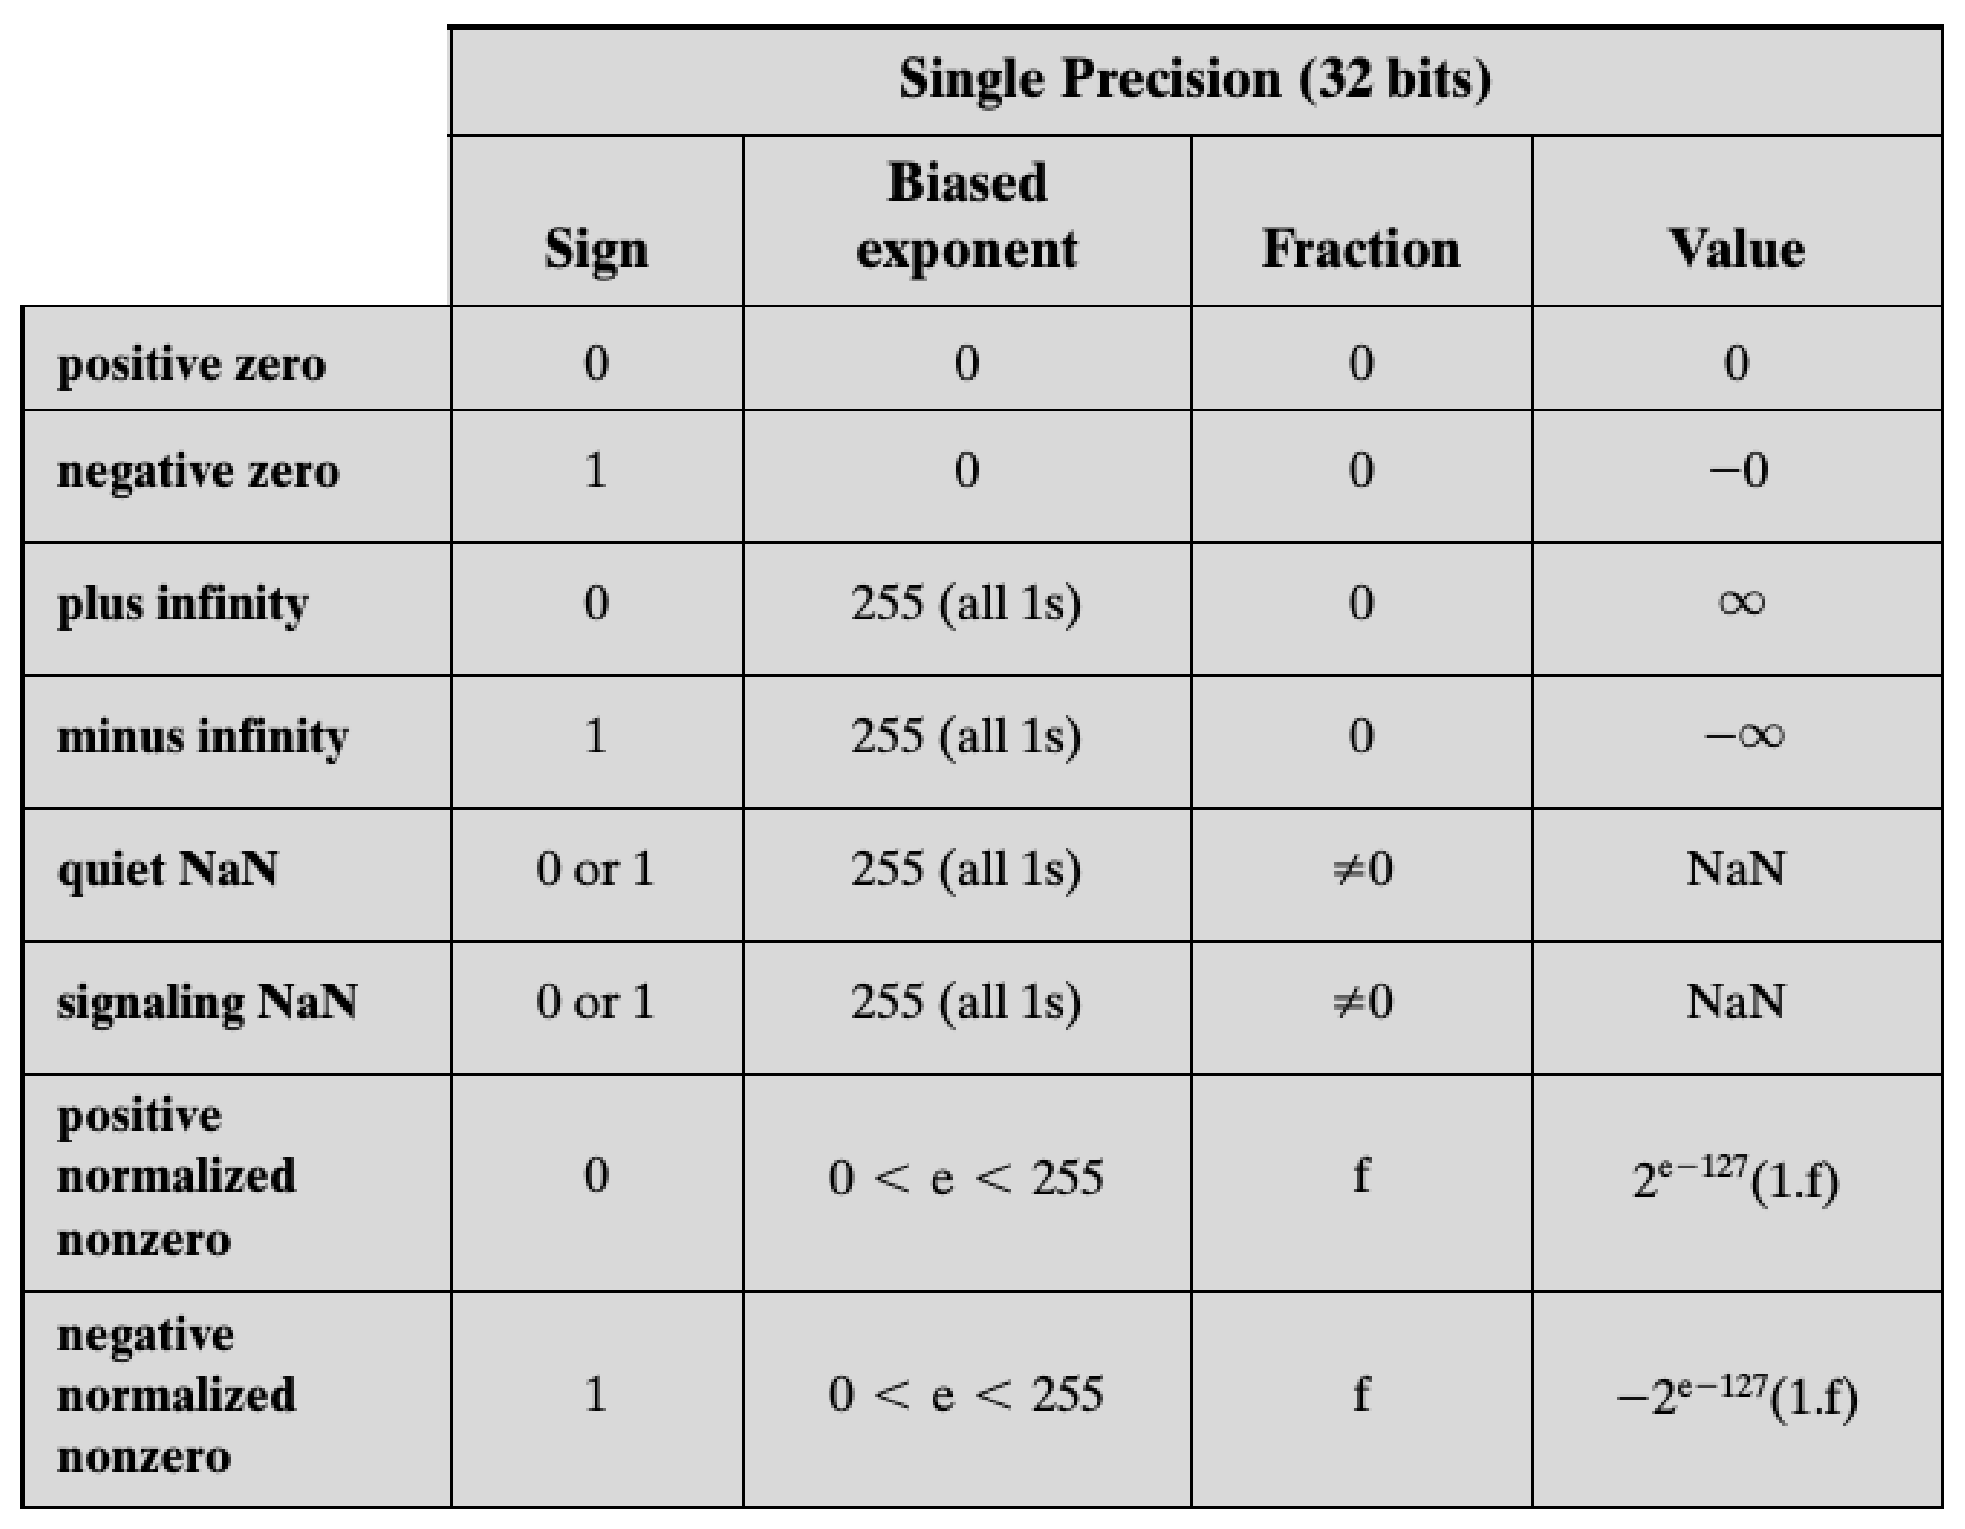
\includegraphics[width=0.7\textwidth]{images/flutuantelimites32.eps}
\end{center} 
\end{frame}

%%%%%%%%%%%%%%%%%%%%%%%%%%%%%%%%%%%%%%%%%%%%%%%%%%%%%%%%%%%%%%%%%%%%%%%%%%%%%%%%%
\begin{frame}{Divisão de números inteiros positivos}
\begin{center}
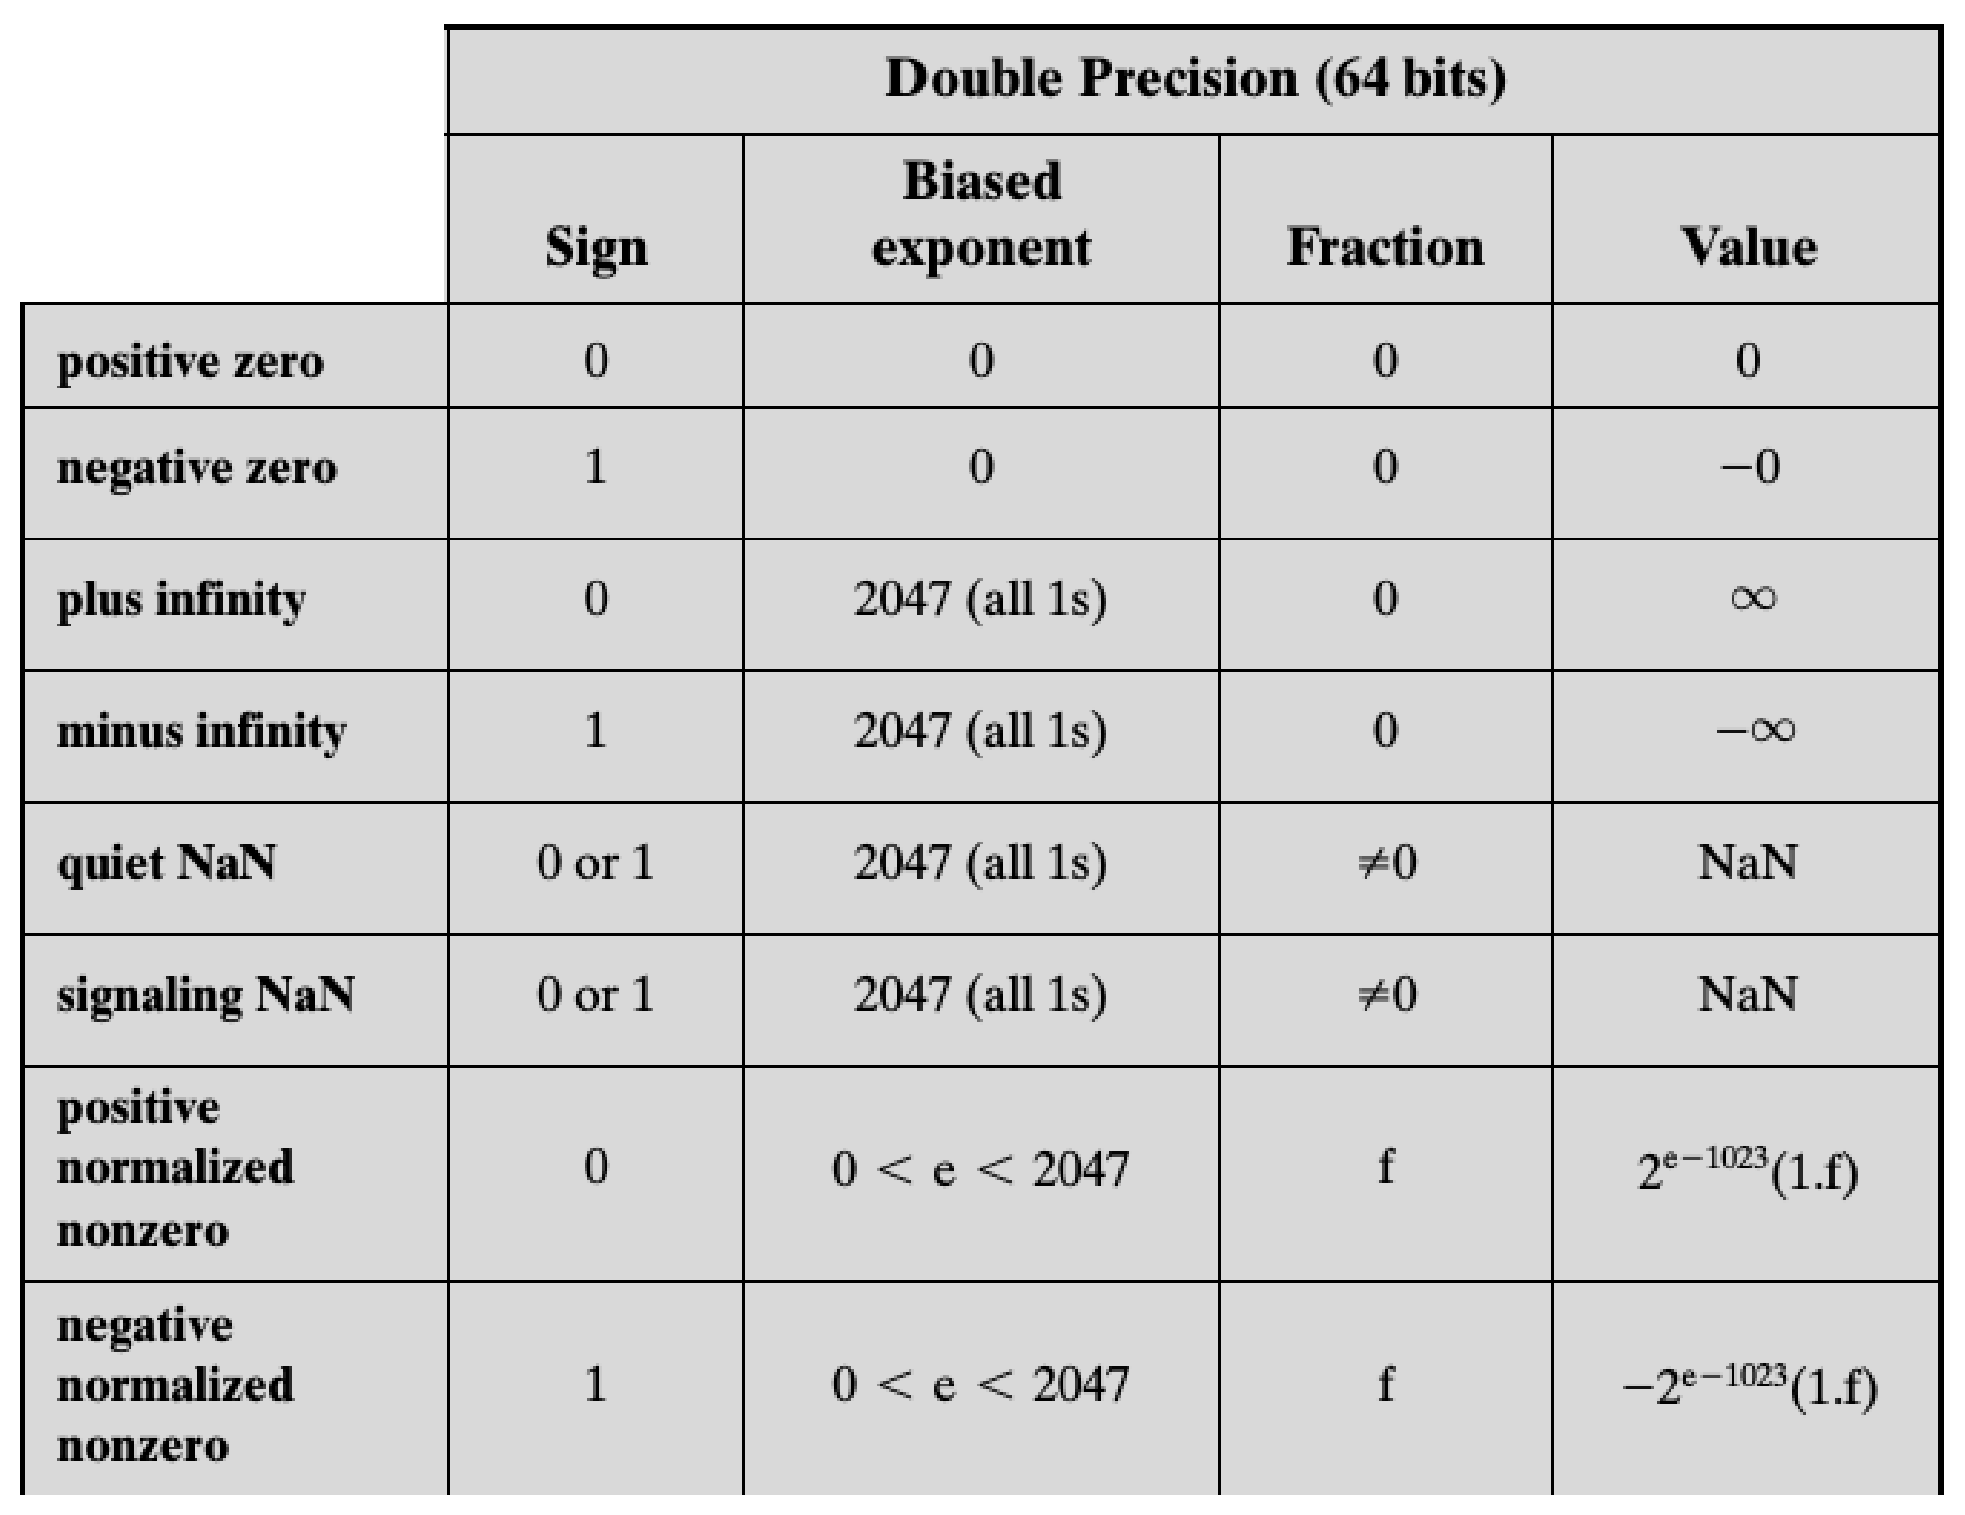
\includegraphics[width=0.7\textwidth]{images/flutuantelimites64.eps}
\end{center} 
\end{frame}


%%%%%%%%%%%%%%%%%%%%%%%%%%%%%%%%%%%%%%%%%%%%%%%%%%%%%%%%%%%%%%%%%%%%%%%%%%%%%%%%%
\begin{frame}{Divisão de números inteiros positivos}
\begin{center}
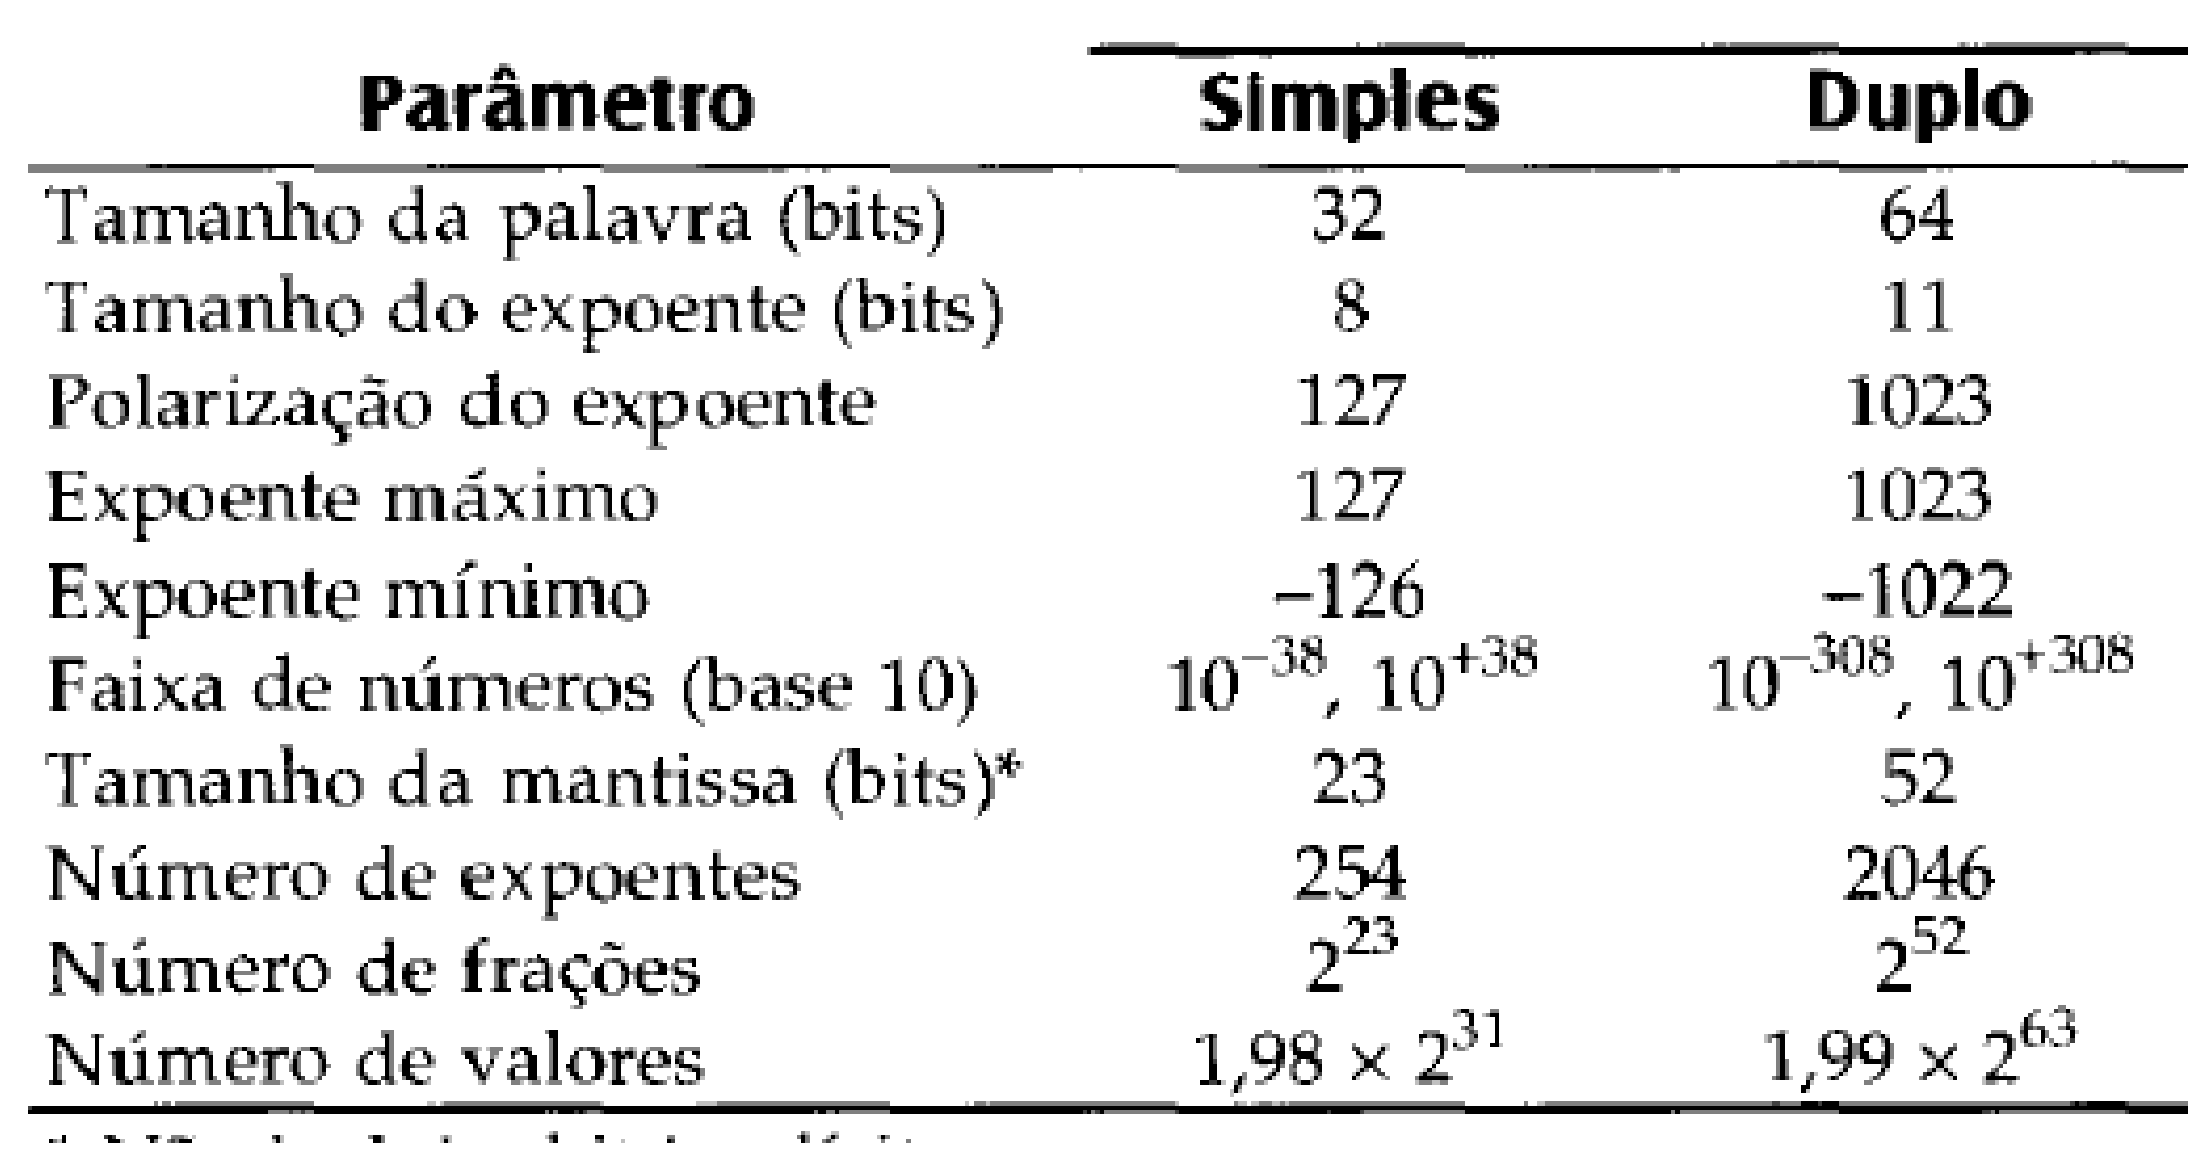
\includegraphics[width=0.9\textwidth]{images/flutuantelimites.eps}
\end{center} 
\end{frame}

%%%%%%%%%%%%%%%%%%%%%%%%%%%%%%%%%%%%%%%%%%%%%%%%%%%%%%%%%%%%%%%%%%%%%%%%%%%%%%%%%
\begin{frame}{Divisão de números inteiros positivos}
\begin{center}
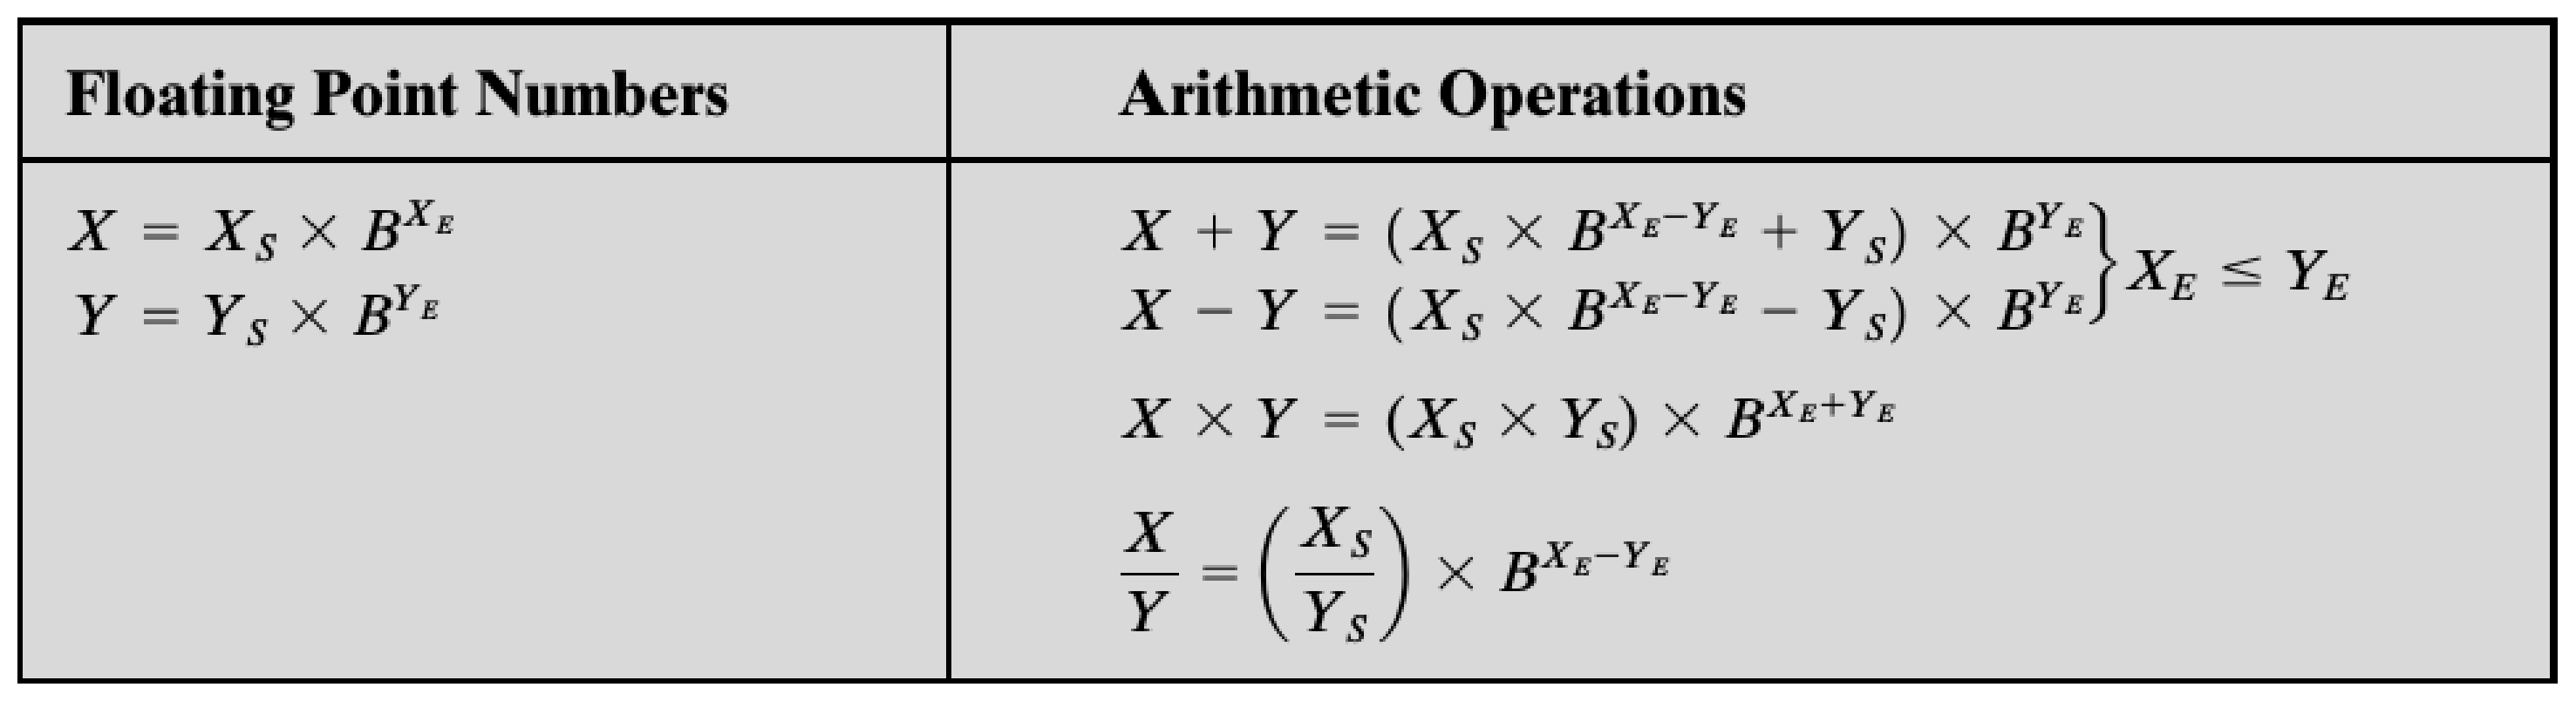
\includegraphics[width=0.9\textwidth]{images/operaciones.eps}
\end{center} 
\end{frame}


%%%%%%%%%%%%%%%%%%%%%%%%%%%%%%%%%%%%%%%%%%%%%%%%%%%%%%%%%%%%%%%%%%%%%%%%%%%%%%%%
\begin{frame}[allowframebreaks]
        \frametitle{References}
        \bibliographystyle{plain}
\bibliography{aritmetica}
\end{frame}



\end{document}
